\chapter{Theoretical Appendix B: Metaphysical Arguments}


If one objects that these are not properly ``biological" considerations, I can only respond by saying that this is no longer the case, if it ever were. What I have called here the \hyperref[SBE]{"Systems Biology Encounter"} (SBE) has made plain the reality described by the great German-American philosopher of science Nicholas Rescher as follows:

\begin{longquote}
The ramifications and implications of philosophical contentions do not respect a discipline's taxonomic boundaries. And we all too easily risk losing sight of this interconnectedness when we pursue the technicalities of a narrow subdomain. In actuality, the stance we take on questions in one domain will generally have substantial implications and ramification for very different issues in other, seeming unrelated domains. And this is exactly why systematization is so important in philosophy - because the way we \textit{do} answer some questions will have limiting repercussions for the way we \textit{can} answer others. We cannot emplace our philosophical convictions into conveniently delineated compartments in the comfortable expectation that what we maintain in one area of the field will have no unwelcome implications for what we are inclined to maintain in others.
\cite[p.97]{Rescher2005}
\end{longquote}

The introduction of ``Systems" methods (mainly drawn from various branches of the complexity sciences) has forced us to contend with the ``implications and ramifications" of the methodological, epistemological, and metaphysical contents of the scientific traditions they are drawn from. If we do not understand what some sophisticated mathematical method assumes about the system to which we apply it, we are bound to make errors in doing so, and we cannot know what ``limiting repercussions" the use of these methods to answer some questions will have for future investigations\footnote{These ``limiting repercussions" are not limited to a restriction in the kinds of methods that can consistently be used, given some particular ``systems biological" approach. If we make no effort to understand these repercussions, we run the risk of having an internally contradictory or degenerate research program, with all of the associated wastages and opportunity costs.}. To fail to take heed of this is simply to concede that we do not really care about ensuring that what we say makes sense, that it is not contradictory, spurious, or simply meaningless. Refusing to make this concession, and lacking any intuitive genius that would allow me to procede without an carefully laid plan, I have made resort to borrowings from philosophers, mathematically- and theoretically-inclined biologists, statisticians, and so forth, to formulate one. I have attempted to do so in a disciplined way; my intent here is not to obfuscate with unnecessary philosophical speculation, but rather to clearly document the conceptual background used to tackle this particular problem in its context.

The meta-method I outline in this chapter assumes that \hyperref[traditions]{Paul Feyerabend's view of science} as a constellation of different \textit{traditions} as substantially correct. This is no longer a particularly contentious view- for the molecular biologist confronting the profoundly foreign, esoteric, and opaque utterances of mathematicians and physicists from the complexity sciences, it is a lived reality. I also accept Feyerabend's contention that historical scientific development occurs \textit{counterinductively}, when traditions show up one another's implicit natural assumptions and metaphysical content. By doing so, scientific traditions make available new ways to think about natural phenomena. I have used this basic view to structure my approach- my objective is to proceed in a way that maximises the counterinductive potential of the historical moment.

The meta-method itself consists in analysing the appropriate ``metascientific unit" of molecular biological practice, the \hyperref[EHJMEx]{Extended Heterogenous Joint Mechanistic Explanation (EHJMEx)}, Melissa Fagan's JMEx concept \cite{Fagan2015} slightly modified, and extended in time to allow accounting for the development of explanations over several different primary papers. By doing this with a \hyperref[agentmodel]{counterinductive general model} in mind, I hope to reveal some of the ``metaphysical ingredients" implied by Harris' explanation and its models, and to suggest how different ones might provide better approaches.

The general modelling approach I have chosen conceives of cells as a type of semiotic agent. This agent-based modelling approach allows the traditional models of population-level stem cell modelling to be expressed as a subset of the larger global model. This in turn permits models with different global metaphysical implications to be compared for local explanatory value. Because the claims I make revolve around the validity of these comparisons, I have explained and defended this at some length.

I have subsequently documented the most important mathematical, methodological and metaphysical ``ingredients" present in Harris' explanations and in my own. I have attempted to place these within the context of the \hyperref[SBE]{SBE} and offer some remarks regarding the epistemological basis of statistical generalisations of complex systems to make this more meaningful for the biologist reader.

Finally, I have made an \hyperref[limits]{attempt to assess the relative sustainability} of the different approaches to systems modelling implicated by this discussion, as first attempt to guide a research program with an explicitly scientific, realistic futurology in mind, relying heavily on Nicholas Rescher's explications of the practical and in-principle limits of scientific and technical progress.

I have sought to make this chapter useful for my own future reference, and for any colleagues coming out of various parts of the molecular biology tradition, who are by now confronted with an astonishing variety of ways to interpret biological phenomena, and few clear guidelines on how they might structure their research programs in light of the SBE. It is nevertheless, by necessity, confined to considerations relevant to retinal stem cells in zebrafish. Due to the limited space and time available, I have made what historians and philosophers of science probably should consider gross oversimplifications. I consider my overall line of reasoning here to be merely one way to ``tell the story" of what is happening to us as biologists, in a way that seems to provide a productive way to think about this problem.

 As I have indicated in this chapter, I intend it in the spirit of what Feyerabend called \hyperref[open]{"open exchange"}-  I do not intend to dictate the terms of future scientific exchange, or to replace one model with another, but rather to suggest one possibility for how we might compare explanations and responsibly guide research programs given the complexity of the present and the uncertainty of the future.

\subsection{Metaphysics, Epistemology}
 Throughout this chapter, I have used the terms ``metaphysics" and ``epistemology" in reference to assumptions, axioms, postulates, etc. about reality and knowledge, respectively. The asking of a question within the natural sciences always has background propositions from both of these domains that are required to make sense of any answer. That is, in order to perform any experiment, we must start with some idea about what sort of thing a phenomenon could consist of (eg. we decide a cell consists mainly of macromolecular consituents arranged in space-time, which informs the methods we use to study cellular life), as well as an idea of what a good answer might be (we must have a sense of how our explanations correspond to reality).
 
 As Nicholas Rescher notes, speaking here of metaphysical issues specifically:
 
 \begin{longquote}
 Metaphysical issues are thus 'basic' or 'fundamental' because they are the product of a methodological stance that facilitates empirical inquiry rather than being a product of our observational study of nature. What those principles of traditional metaphysics do is to provide question-generic presuppositions of factual inquiry. Natural science (physics, as the Greeks called it) provides the specific answers to our specific questions. But metaphysics is a matter of 'first principles': it sets out the presuppositional framework within which those answers are developed.
 \cite[p.4]{Rescher2000}
 \end{longquote}
 
Rescher further subdivides metaphysics into two broad categories:

\begin{longquote}
Presuppositonal inquiry in relation to science has two aspects, depending on whether we ask, 'What presuppositions are called for if we are to do science \textit{at all}?' or 'What presuppositions are called for if we are to do science the particular way in which the course of experience has ultimately taught us to proceed?' Those initial most fundamental principles are fixed. But then the less fundamental implementation is something else again, something learned, something in relation to what the case of experience costs. At this less fundamental level the presuppositions and methodological principles of natural science must be retrospectively informed and restructured in the light of the deliverance of scientific agency itself. (At this stage we can usefully resort to Otto Neurath's graphic image of the boat refitted and repaired while sailing in the open sea.) At this level of consideration metaphysics not merely underpins but also reflects science. \cite[p.5]{Rescher2000}
\end{longquote}

It is the latter, lesser category of metaphysical proposition I am interested in here, and it is this sort of theoretical ``at-sea" refit that I am attempting to conduct by considering the metaphysical and epistemological implications of biological theory in the light of our lived experience of scientific practice.

\subsection{Bayesian Epistemological View on Statistical Generalisation}
\label{sec:BayesEpistemology}
I have chosen to make extensive use of Bayesian statistical methods\footnote{Some would describe them as Laplacian, since Laplace famously provided their first real scientific use in calculating the posterior distribution of the mass of Saturn; Bayes was calculating lottery chances. Properly speakin, Laplacian statistics are the original statistical orthodoxy }, which have by now matured into a useable toolkit for the cellular and molecular biologist. While Bayesian statistics are sometimes portrayed as a marginal subjectivist trend, to be ignored by serious biostatisticians, nothing could be farther from the truth. 

Under




\section{Study Structure in the Light of Tradition}

A scientific report is, by its nature, a retrospective structuring of an investigation. Structuring a scientific study requires defining the goals and methods of the study. To the extent that the products of a research program (eg. the intellectual output of a number of labs over some period of interaction) are structured by some common set of rules for determining their goals and methods, these rules turn out to be surprisingly difficult to define. As the Kuhnian philosopher of science Philip Kitcher noted about the teaching of classical genetics:

\begin{longquote}

Neophytes are not taught (and never have been taught) a few fundamental theoretical laws from which genetic ``theorems" are to be deduced. They are introduced to some technical terminology, which is used to advance a large amount of information about special organisms. Certain questions about heredity in these organisms are posed and answered. Those who understand the theory are those who know what questions are to be asked about hitherto unstudied examples, who know how to apply the technical language to the organisms involved in these examples, and
who can apply the patterns of reasoning which are to be instantiated in constructing answers. More simply, successful students grasp general patterns of reasoning which can be used to resolve new cases. \cite{Kitcher1984}

\end{longquote}

It is the effective use of these patterns of reasoning that constitutes the good or proper practice of biology. The neophyte biologist, if he inquires into the general structure of those patterns, is likely to be met with what Paul Feyerabend referred to as the ``fairy-tale" underlying the special credibility afforded natural scientists:

\begin{longquote}

Scientists have ideas. And they have special methods for improving ideas. The theories of science have passed the test of method. They give a better account of the world than ideas which have not passed the test. \cite{Feyerabend1993}

\end{longquote}

This is an appealing myth, particularly for the learner motivated by a search for the truth, which may account for its use in redirecting the student to immersion in experimental practice. We often teach that there is actually only one method, ``The Scientific Method" (hereafter Method), which consists in iteratively falsifying hypotheses about phenomenal reality, allowing a model of that reality (in the form of an logical argument constructed of these hypotheses) to be refined over time so that the model is, by correctly applying this procedure, inexorably brought closer to reality\footnote{This instruction, strangely, often fails to note the origin of this notion with Karl Popper and its subsequent uneven reputation as a good description of, or prescription for, scientific activity. This idea now often goes by the name of ``evolutionary epistemology", with the general idea being that incorrect hypotheses are selected against in a progressive refinement of knowledge. To whatever extent this happens, the selective procedure is not iterative application of a particular methodology or set of rules.}.

The conscientious student, looking for serious academic treatments of the Method, is immediately forced to contend with a bewildering array of perspectives on what constitutes the Method and what procedures are legitimately employed in properly Scientific practice. Most of these are produced from accounts of the development of physics and its auxiliary sciences. Many insist that the Method consists of some formal criterion or procedure which is plainly not in use in biology or in scientific practice at large. The wide disagreement on the very concept of any such Method has, at least, the salutory function of disabusing the student of the notion that scientific practice could possibly be governed by the well-understood ``special methods" of Feyerabend's ``fairy-tale" scientists.

Deprived of any ``special method" recipe to apply to his problem, the biologist only has resort to the patterns of reasoning in their field. These are normally understood heuristically or intuitively- we know how to make arguments about molecular systems without any training in formal logic, and without necessarily offering any account of \textit{what we are doing} when we are making the argument. This type of understanding is sufficient when one is simply applying these patterns to new cases. What are we to do when confronted with claims by a colleague who is using novel, foreign, imported, etc. scientific methodologies? We may attempt to ``muddle through" by ``seeing what works", but this concedes entirely too much to influences we generally understand to be orthogonal to systematisation of knowledge about nature. If ``what works" is largely defined by what gets published, the result of ``muddling through" without clear method will frequently be shaped more by the parochial interests involved in the scientific process than by the drive for better biology\footnote{For instance, both the academic careers of scientific personnel staffing with granting agencies and editorial boards, and the commercial success of manufacturers selling expensive scientific equipment, reagents etc. depend directly on the perception that the methodology used by the personnel with the equipment and reagents is in some way \textit{orthodox}. This perception may be justified with reference to some philosophical rule to establish the boundary between science and non-science, such as Popper's ``pseudoscience" demarcation. In the particular case of stem cell biology, as Melissa Fagan has noted, even basic conceptual divisions (eg. ``adult" vs. ``embryonic" stem cells) can become politically charged \cite[p.47]{Fagan2013}. Given the lucre associated with promising approaches to stem-cell based regenerative medicine, the influence of these ``orthogonal influences" is particularly strong in the SCBT- the perception that a particular theoretical approach undergirding some therapy is mainstream, well-supported science is critical for the therapy's adoption.}.

The student may therefore return to academic discussion of scientific practice looking not for any recipe-Method, or indeed systematic prescriptions about how to structure studies and analyse data, but simply for points of agreement on what science is and what scientists are doing. As a full survey of this literature would extend across a huge range of studies in a variety of disciplines, I have instead focused on one informative point of agreement arrived at in the philosophy of science. In the second half of the 20th century the observation was made by Thomas Kuhn, Paul Feyerabend, Imre Lakatos, and others, that science plainly did not proceed by iterative hypothesis falsficiation, as asserted by the more credible scientific realists of the first half of the 20th century. Kuhn, Feyerabend, and Lakatos conceived of different scientific ``paradigms", ``traditions", or ``research programmes", respectively, making competing claims on truth in a historical process of scientific development. Rather than collectively producing one huge cultural artefact called ``Science", it became clear that the only way to explain the apparently ``revolutionary" character of science, as well as the chaotic succession of different scientific theories, was to understand science as the activity of people committed to a plurality of different methodologies interacting in particular historical contexts.

These ideas and their relation to one another took time to digest, but by the end of the 20th century, most philosophers of science agreed that scientific theories must be analysed in their historical, social, and intellectual context, and that diverse scientific schools of thought advance theories and models as competing explanations for phenomena, rather than proceeding by any mutually agreed upon Method. Scientists participate in and draw from these schools as they perform their work, convert from one school of thought on an issue to another as the latter becomes more fleshed-out and persuasive, and so on. From a biologist's perspective, this is a realistic description of scientific practice as a type of ecosystem, rather than the rote application of some logician's rules. The agreement of the philosophers suggests that this is genuinely a better description of what scientists are actually doing than the quasi-mythological ``received view" of the past, particularly in the context of the bitter disputes on virtually every other topic.

I have therefore chosen to define a framework derived from these basic insights in order to concretely examine what I take to be the leading research program in my field. In order to structure this examination, I have chosen to make use of a number of concepts from the philosophy of science: Feyerabend's ``tradition", Fagan's ``Joint Mechanistic Explanation (JMEx)", the latter modified by Schaffner's ``extended theory". I briefly describe some of the relevant background of these concepts with occasional clarifying examples from our field. I then make modifications to these concepts for my own use and demonstrate how they inform the structure of this study.

\subsection{Feyerabend's Scientific Traditions}
\label{traditions}
The central, seminal insight of Paul Feyerabend's \textit{Against Method} is that the observed succession of scientific theories occurs by counterpositional advancement of incompatible opposing theories, because only counterinductive comparisons \textit{between} theories are capable of showing up their implicit assumptions and allowing them to be challenged. Feyerabend explains:

\begin{longquote}

... it emerges that the evidence that might refute a
theory can often be unearthed only with the help of an incompatible
alternative: the advice (which goes back to Newton and which is still
very popular today) to use alternatives only when refutations have
already discredited the orthodox theory puts the cart before the
horse. Also, some of the most important formal properties of a theory
are found by contrast, and not by analysis. A scientist who wishes to
maximize the empirical content of the views he holds and who wants
to understand them as clearly as he possibly can must therefore
introduce other views; that is, he must adopt a \textit{pluralistic methodology}.
He must compare ideas with other ideas rather than with
'experience' and he must try to improve rather than discard the views
that have failed in the competition.\cite[p.20]{Feyerabend1993}

\end{longquote}

\textit{Against Method} takes as its historical exemplar Galileo's advancement of the heliocentric Copernican model against its orthodox Aristotlean competitor championed by the Catholic Church. Although we commonly think of the so-called Copernican Revolution as the replacement of an obviously defective theological explanation by a properly formed theory from the empirical sciences, Feyerabend shows that this conceals the actual means by which Galileo makes his persuasive case for the (itself badly defective) Copernican model. Centrally, it is process of comparing the heliocentric and geocentric theories that makes the implicit, unstated ``natural assumptions" of the geocentric theory clear. Feyerabend elaborates on the kind of structures that counterinduction can reveal:

\begin{longquote}

Methodological rules speak of 'theories', 'observations' and 'experimental results' as if these were well-defined objects
whose properties are easy to evaluate and which are understood in
the same way by all scientists.

However, the material which a scientist \textit{actually} has at his disposal,
his laws, his experimental results, his mathematical techniques, his
epistemological prejudices, his attitude towards the absurd consequences of the theories which he accepts, is indeterminate in many
ways, ambiguous, \textit{and never fully separated from the historical background}. It is contaminated by principles which he does not know
and which, if known, would be extremely hard to test. Questionable
views on cognition, such as the view that our senses, used in normal
circumstances, give reliable information about the world, may invade
the observation language itself, constituting the observational terms
as well as the distinction between veridical and illusory appearance.
As a result, observation languages may become tied to older layers of
speculation which affect, in this roundabout fashion, even the most
progressive methodology. (Example: the absolute space-time frame
of classical physics which was codified and consecrated by Kant.)
The sensory impression, however simple, contains a component that
expresses the physiological reaction of the perceiving organism and
has no objective correlate. This 'subjective' component often merges
with the rest, and forms an unstructured whole which must be
subdivided from the outside with the help of counterinductive
procedures. (An example is the appearance of a fixed star to the
naked eye, which contains the effects of irradiation diffraction,
diffusion, restricted by the lateral inhibition of adjacent elements of
the retina and is further modified in the brain.) Finally, there are the
auxiliary premises which are needed for the derivation of testable
conclusions, and which occasionally form entire \textit{auxiliary sciences}.

...

Consideration of all these circumstances, of observation terms,
sensory core, auxiliary sciences, background speculation, suggest
that a theory may be inconsistent with the evidence, not because it is
incorrect, \textit{but because the evidence is contaminated}. The theory is
threatened because the evidence either contains unanalysed sensations which only partly correspond to external processes, or because
it is presented in terms of antiquated views, or because it is evaluated
with the help of backward auxiliary subjects.

...

It is this \textit{historico-physiological character of the evidence}, the fact that it
does not merely describe some objective state of affairs \textit{but also
expresses subjective, mythical, and long-forgotten views} concerning this
state of affairs, that forces us to take a fresh look at methodology. It
shows that it would be extremely imprudent to let the evidence judge
our theories directly and without any further ado. A straightforward
and unqualified judgement of theories by 'facts' is bound to eliminate
ideas \textit{simply because they do not fit into the framework of some older
cosmology}. Taking experimental results and observations for granted
and putting the burden of proof on the theory means taking the
observational ideology for granted without having ever examined it.

\cite[p.52]{Feyerabend1993}
\end{longquote}

Feyerabend argues that it was the cognitive contrast between the Copernican model and orthodox Aristotlean geocentric and geostatic conceptions which showed up precisely this kind of implicit assumption. In this case, the assumption in question gave rise to the unchallengeable ``fact" that the Earth could not be moving rapidly through space because objects are observed to fall straight down- if the Earth were in motion, falling objects would appear to be moving in a slanting trajectory.

\begin{longquote}
We start with two conceptual sub-systems of 'ordinary' thought ... One of them regards motion as an absolute process which always has effects, effects on our senses included.
The description of this conceptual system given here may be somewhat
idealized; but the arguments of Copernicus' opponents, which are
quoted by Galileo himself and, according to him, are 'very
plausible', show that there was a widespread tendency to think in its
terms, and that this tendency was a serious obstacle to the discussion
of alternative ideas.

...

The second conceptual system [the Copernican model] is built around the relativity of
motion, and is also well-entrenched in its own domain of application.
Galileo aims at replacing the first system by the second in \textit{all} cases,
terrestrial as well as celestial. Naive realism with respect to motion is
to be \textit{completely eliminated}.

...

Viewing natural phenomena in this way leads to a re-evaluation of all
experience, as we have seen. We can now add that it leads to the
invention of a \textit{new kind of experience} that is not only more sophisticated
\textit{but also far more speculative than} the experience of Aristotle or of
common sense. Speaking paradoxically, but not incorrectly, one may
say that \textit{Galileo invents an experience that has metaphysical ingredients}. It
is by means of such an experience that the transition from a geostatic
cosmology to the point of view of Copernicus and Kepler is
achieved.

\cite[p.69]{Feyerabend1993}
\end{longquote}

In other words, the conceptual frame of the Galilean observer has shifted so that fundamental, common-sense natural perceptions (objects which are not observed to be in motion cannot be in motion) are overturned, and ``experience now ceases to be the unchangeable fundament which it is both in common sense and in the Aristotelian philosophy.
The attempt to support Copernicus makes experience 'fluid' in the
very same manner in which it makes the heavens fluid, 'so that each
star roves around in it by itself'. An empiricist who starts from
experience, and builds on it without ever looking back, now loses the
very ground on which he stands." \cite[p.72]{Feyerabend1993}

Thus, the Copernican Revolution succeeded because the counterinductive comparison of the older Aristotlean explanation with Galileo's theory revealed the flawed natural assumption of the geostatic model- the assumption that all motion is operative, that objects not in apparent motion for some observer are indeed at rest in an absolute sense. Only by thinking of motion as a relative phenomenon that only produces observable effects when bodies are moving \textit{with respect to one another}, does the problem with the assumption of absolute motion become obvious.

This success was not the result of any of the usual ``rules" offered as candidates for the mono-Method. Galileo's theory substantially contradicted the available evidence, erroneously asserted the reliability of telescopic observations, made extensive use of ad hoc hypotheses, and was advanced by propagandistic and even dishonest means. Much of this was unavoidable. Ad hoc hypotheses are necessary for new theories because the auxiliary sciences associated with them have not been developed- scientific development is intrisically uneven, obligating the use of these makeshift theoretical devices. Without a certain level of dishonesty and rhetorical sleight of hand on Galileo's part, the Copernican program would have succumbed to the greater development and argumentative weight of the scholastic tradition. As Feyerabend notes, if any of the typically suggested Method criteria were applied, the Church would have won the debate and we might still have an Aristotlean cosmology!

For Feyerabend, then, science, like other human social practices (including the arts, administration, and so on) consists of a variety of interacting traditions with differing assumptions, methods, sensory interpretations, and so on. The development of science is thus ``not the interaction of a practice with something different and external, \textit{but the development of one tradition under the impact of others.}" \cite[p.232]{Feyerabend1993}

\subsection {Classical and Molecular Genetics: Shared Traditions, Plural Methodologies}
\label{PS}
To bring the implications of Feyerabend's views into some familiar relief, let us briefly examine a case from the field: the ``molecularisation" of zebrafish genetic experimentation. Because the zebrafish genome took some time to be released in reliable revision, the use of the Mendel/Morgan ``classical genetic tradition" (CGT) was widespread in mapping experiments before this. One might locate an allele of interest by recombination experiments, mapping its position in (by now unfamiliar) units of centimorgans to reflective relative recombination frequency between loci. This is, of course, increasingly unusual, as the practices of the Watson/Crick ``molecular genetic tradition" (MGT) are more and more accessible due to the previously unavailable genomic data\footnote{It can be an edifying experience to ask a student to ``convert" between CGT units like centimorgans and MGT units like megabases. At the very least, the cognitive discomfort produced will tend to reveal a problem in the question's assumptions to the student. At best, one can gain a practical understanding of how scientists make sense of and experience ``switching" between different traditional explanatory frames.}. The zebrafish geneticist now has access to two traditions to perform their work, and will make recourse to either as they assess circumstances warrant (without any reference to an explicit external rule about which tradition should supercede the other in particular cirucmstances). For instance, if I am planning to cross two fish that are heterozygous at some allele, I will use typical CGT assumptions to calculate the expected number of various offspring genotypes. Even if I was able to offer a reasonable description, in molecular terms, of zebrafish meiosis, recombination, fertilisation, and so on, I would never choose to do so- an MGT explanation is unnecessary where Mendel's laws suffice, and will begin to lack explanatory power the moment I apply it to another species, unlike the Mendellian CGT framework.

One might object that the claims of the CGT tradition ``reduce" in some meaningful way to the MGT tradition, or ``cover" for it, so that CGT theories are in fact just abstractions of MGT theories. In other words, the fact that MGT claims are not useful and lack explanatory power in some areas does not change the fact that MGT \textit{could} provide good theoretical explanations for all of the claims of CGT. As Kitcher shows, this is not correct\footnote{Kenneth Schaffner later insisted that Kitcher was wrong, and that CGT theories are reducible to MGT theories, because the MGT theories establish direct linkages between DNA sequences and proteins, and thus are formally equivalent to the classical concepts of genes and phenotypes \cite{Schaffner1993}. This now seems obviously mistaken on at least 2 counts: (1) there is no stable molecular entity implicated by ``the gene": its local context in terms of primary sequence (promoters etc.), and tertiary arrangement in a nuclear ``transcription factory", all contribute to the complexity of the causal locus involved in transcription alone, and (2) there are very few phenotypes of interest that are caused by stable, uncomplicated interactions between DNA and protein such that classical genetic phenotypes reduce cleanly or usefully to descriptions solely in terms of macromolecules. Moreover, this does not address Kitcher's point: there \textit{are} phenotypic traits which are \textit{not} describable in terms of their protein constituents, and that there \textit{are} higher-level processes which may be generated by any number of configurations of molecular consituents and are thus better understood as types of processes and not as specified molecular systems.}. The CGT description of the \textit{process} of meiosis as a particular type in which ``paired entities (i.e. chromosomes) are separated by force so that one member of each pair is assigned to a descendent entity"\cite[p. 349]{Kitcher1984} (which Kitcher calls a PS-process), is not describable solely in terms of the molecules participating in the process. Because a PS-process like meiosis can be realised in any number of ways at a molecular level, PS-processes cannot be accounted for in a general way by MGT theories. The manner in which different traditions frequently address different levels of biological organisation in similar non-interchangeable ways is discussed further below.

We can extend this example to see that the typical biologist has access to a great plurality of methodological traditions. Biologists are intuitively used to ``translating" between traditions and to switching freely between them when translations are cumbersome or useless. Where there are no deep conflicts between the implict aspects of these traditions, no counterinductive process occurs. That is, we do not ``refute" CGT with MGT in the same way the Copernican Revolution ``refuted" Aristotlean geostatic theory because MGT rarely makes the structure of CGT seem untenable to us; an attempt to replace CGT with MGT would surely be quixotic. We simply appropriate the methodology of the tradition which is most appropriate for the problem at hand.

\subsection{Sense of ``Tradition" in this study}

Thomas Kuhn was soundly criticised for the vague sense in which he used the term ``paradigm"\cite[p.206]{Schaffner1993}, which left him unable to offer coherent explanations. Feyerabend was far more precise, but, as a philosopher rather than a practitioner, never had need (or desire) to guide a scientific project from within the worldview he developed. Having erected an unassailable proof that no special Method existed, and that subscribing to one would have prevented the central Galilean vignette of naive philosophy of science's core Enlightenment self-narrative, he effectively retired\footnote{Feyerabend's chilly reception and subsequent exile is difficult to understand in retrospect, as the basic framework of his argument is now generally understood to be correct in some sense or another. Whether one ascribes the initial poor reaction to his combative personality or flamboyant political statements, his ideas are by now pervasive, even normative. The appearance of ``post-colonial" biological studies would have been very unlikely in the Popperian scientific world of the 1960s. Curiously, the Feyerabendian molecular biological traditionalist will note that this may actually constitute an intra-traditional ``colonial" venture on the part of critical theorists and continental philosophers.}.

When Feyerabend wrote of ``scientific traditions", he meant scientific practice in its broadest possible sense, a social practice with ``historico-physiological character". That is, scientific theories are conditioned by the historical moment, and by the involvement of the observer and their social, cognitive, and biological baggage in the phenomenon under study. For the purposes of making Feyerabend's arguments against the existence or advisability of a mono-Method, this was entirely adequate, but I intend only to deal with a limited subset of these materials. The ``Stem Cell Biological Tradition" defined below, in its full Feyerabendian sense, includes rumours circulated at stem cell conferences, methodological tips and tricks passed on by observation of careful practice (that could never be learned from any protocol), the commercial aspirations of particular academics, and so forth, in addition to all of the ``properly scientific" materials implicated by all of the publications that have ever used the ``stem cell" concept or a recognisable homologue. While my use of the term acknowledges this broader contextual sense, I will only look at the explicitly documented ``traditional background" of particular, formally advanced explanatory statements or models. The objective here is mainly to account for molecular biological explanations occuring within a ``composite tradition" with diverse, only partially overlapping internal ``subtraditional" currents.

Therefore, in general, I have not intended to draw any hard divisions between subtraditional currents in the molecular biological tradition (MBT). While I have pointed out how MBT explanations may include components drawn from irreducibly separate subtraditions (the irreducible CGT explanation for PS-processes discussed \hyperref[PS]{above}), I have only mentioned the philosophical, methodological, etc. implications of MBT subtraditions where necessary, as the primary concern is the extra-traditional background of the ``systems" modelling approaches encountered in the data chapters. For instance, in the case of the Galton-Watson branching process model, my definition of this as an artefact (one can think of a probability distribution plot figure in a paper) from the Probability Theory Tradition (PTT) means that this is a traditional statistical solution to an early biological lineage model, which stands in for the large-scale behaviour of a simple model of lineage growth and extinction, in a larger MBT mechanistic explanatory framework (the \hyperref[EHJMEx]{MEx}, Mechanistic Explanation).

I have also made reference to the ``Stem Cell Biological Tradition" (SCBT), which is intended to convey the last approximately 6 decades of research practice organised around the stem cell concept\footnote{I include anti-stem cell and stemness theories in this tradition, since they are marginal heresies to a hegemonic orthodoxy and not meaningfully independent.}. The question of the relationship between the MBT and SCBT is not simple. Till and McCulloch were not offering molecular mechanisms for the phenomena they were documenting \cite{McCulloch1960}, and could well have been described as operating in an earlier Cell Biological Tradition (CBT).

 My conception of this relationship is that, generally, SCBT practice has been ``molecularised"; most of the explanations that SCBT practitioners care about are molecular MEx, and the SCBT is therefore a subtradition of the MBT. Nevertheless, the \hyperref[hierarchy]{multilevel} character of all MBT explanations means that SCBT practicioners routinely use CBT concepts where a specified molecular system would be useless or inappropriate. An example is the ubiquitous abstraction of mitotic phenomena as a class of cell behaviour in SCBT explanations (referred to simply as ``mitosis", ``proliferation", ``renewal" etc), rather than making any attempt to specify this central concept in explicitly molecular terms.

 Therefore, in this sense, SCBT practitioners are used to ``slotting in" explanatory components from a variety of traditions in order to offer a broader MEx for some phenomenon (regeneration, repair). We are in this sense classic Feyerabendian ``Epistemological Anarchists", using whatever explanatory frames suit our purposes. This habit has, in the context of the \hyperref[SBE]{SBE}, shifted from predominantly ``intra-" to ``inter-traditional anarchism", with the result that the required level of sophistication required to advance a good molecular MEx has increased steeply.
 
 The SCBT is a particularly notable subtradition of the MBT because of its explicitly therapeutic, and therefore ethical and normative orientation. That is, while the broader developmental biology tradition does not have a unified therapeutic goal, the SCBT is structured by the objective of interacting with stem cell phenomena to medicinal and therapeutic ends. This particularly ethical aspect of the SCBT compels me to make some brief remarks about how my own study's design is be guided by this ethical orientation.
 
\section {EHJMEx as a Subtraditional Metascientific Unit of Molecular Biological Theory}
\label{EHJMEx}

From the practitioner's perspective, we are interested in thinking about the ``metaphysical unit" of scientific practice on a finer scale than allowed by Feyerabend's concept of a tradition. If we take the practice of molecular biology to be about generating explanations for biological phenomena in terms of macromolecules and their organisation, we want to know enough about the structure of these explanations to allow us to compare them. While we know that we are looking for the ``underlying molecular mechanisms" of (usually) cellular phenomena, it is not always clear how we might go beyond intuitive preferences for one proposed mechanism or another in, say, deciding what assay to perform next. We may reason in terms of plausibility or agreement with evidence, but we rarely do so formally\footnote{It may not even be advisable to do so in many cases, as, for instance, we often become aware of problems with particular lines of research which are not disclosed in published reports.}. Moreover, it is sometimes unclear what kinds of descriptions are mechanistic explanations (MEx) and when we can agree such a description has explained some phenomenon.

A deliberate counterinductive evaluation of two ``units" of biological theory that is productive- one that allows us to imaginatively explore the metaphysical implications of two scientific models for explaining some phenomenon- requires a definition of the unit. Feyerabend's description of scientific tradition suggests that we start by looking at ``local" traditional practice. I have thus chosen here to rely heavily on a general conception of the ``locally accepted method" proffered by the philosopher of stem cell biology, Melinda Bonnie Fagan (Fagan hereafter), who has extremely usefully summarised these ideas in her recent book ``Philosophy of Stem Cell Biology: Knowledge of Flesh and Blood", as well as a number of other useful publications\cite{Fagan2013,Fagan2015,Fagan2015a}. I have modified her idea by extending it temporally (following Schaffner's Extended Theory concept\cite[p.211]{Schaffner1993}) and by placing it within the what I take to be the extended context of the Molecular Biological Tradition conceived of in Feyerabend's terms- explicitly including its auxiliary sciences and metaphysical implications.

\subsection{Law-based and Causal Mechanistic Explanations}

Fagan is not the first philosopher of science to note the local currency afforded to MEx in the MBT. Indeed, she has thoroughly addressed the inadequacies of earlier theorisations of biological MEx. In general, philosophers have previously advanced law-based and causal theories to explain what biologists are doing when they offer MEx.

\subsubsection{Law-based MEx}

Law-based theories suggest that MEx operate by explaining a phenomenon in terms of universal, exceptionless laws of broad scope, given some initial set of conditions. I take it to be obvious that this is not what biologists are doing- MEx simply do not express this kind of law, and I have personally never encountered a biologist who understood MEx in anything like ``universal, exceptionless" terms, even as a ``regulative ideal" toward which MEx are asymptotically refined. Mechanistic diversity underlying broad classes of phenomena is understood to be normative, so ``nomological" law-based concepts are of little use to us.\footnote{Fagan refutes recent advocacy of the law-based view. Schaffner previously advocated for a more sophisticated conception in which biological explanations were only ``universal" or ``exceptionless" in the specific context where they were formulated (species, tissue, cell type, etc). Biological explanations might then consist of laws which support counterfactual refutation. As Fagan points out, MEx are not even expected to be locally universal explanations for phenomena. One of the best-understood MEx, that of asymmetric mitosis in drosophila Germline Stem Cells (GSCs), only applies in full to about 80\% of GSC divisions which ``have a plane of division parallel to the hub-GSC binding site."
\cite[p.97]{Fagan2013}
A proponent of the idea that biological theories make use of ``laws" might have resort to ``legal pluralism", in which they assert that more than one law may pertain to a particular case, depending on some contextual factor. I doubt a concept of this sort can really be any more useful than Fagan's Joint MEx description adopted here.
}

\subsubsection{Causal MEx (CauMEx)}
Theories of MEx that are underlain by some understanding of \hyperref[causality]{causal relations} described by the mechanism are more influential than law-based ones within biological practice. The most typical theory of causality taken to underlay these ``Causal MEx" (CauMex, com-ex) is an \hyperref[causality]{interventionist} one, typically expressed in Fagan's description of ``manipulability theory". Indeed, biological studies are often divided between ``interventional" and ``non-interventional", largely along the lines proposed by James Woodward. As Fagan notes of Woodward's description:

\begin{longquote}
This theory analyzes causality as a relation between values of variables, X and Y. X causes Y if and only if there is a possible
manipulation of some value of X, under idealized experimental conditions, such that the value of Y changes. Woodward's is a counterfactual
account of causality, hinging on what \textit{would} happen to the values of
variables in an idealized experiment, or \textit{intervention}. An intervention I
on variable X with respect to variable Y is a causal process that determines the value of X in such a way that, if the value of Y changes, then
the change in Y occurs only in virtue of the change in X.

The concept of an intervention provides a regulative ideal for experiments aimed at discovering causal relations: approximate the conditions
of ideal experimental interventions. Insofar as they meet this standard,
experiments reveal genuine patterns of counterfactual dependence
among sets of entities and their properties, i.e. causal relations in the
world. Because invariance [in the correlative relationship between X and Y] is required only under \textit{some}, not all, interventions, causal explanations need not include general laws. The range
of interventions under which a dependency relation between values X
and Y holds may be broad or narrow. Within their range, 'fragile' dependency relations are no less causal than those with a much wider range of
invariance: universal causal laws. Experiments, if correctly designed,
reveal relations between values of variables that are invariant under
some interventions. The relevant counterfactuals for causal relations are
tested by realizing particular values of X and observing the values of Y
under controlled circumstances that fall within the range of invariance
for X and Y.
\cite[p.99]{Fagan2013}
\end{longquote}

I quote this description at length because it well-describes the essential orthodox view implied when we teach students the canonical experimental typology of the MBT. This is a highly plausible account of how these experiments ``work" to explain the underlying system. We can think of a typical dose-dependence curve in pharmacological research: we apply some hormone over a range of physiologically-reasonable doses X to some cells, and observe the response of some functional readout Y (say, the cell-normalised luminance of a luciferase reporter downstream of a receptor for X). If there is a invariant relationship between X and Y over some reasonable dose range, we may postulate that the application of dose X causes the luminance of the cells Y by resulting in hormone binding, activation of a promoter element, etc. If we perform a series of other interventions we can test counterfactuals about this relationship: we may try to observe the movements of GFP-tagged signalling proteins during the application of dose X, or apply inhibitors of enzymes, antagonists of receptors, and so on, to implicate the other elements involved in the causal chain we suppose makes up the mechanism. Therefore, CauMEx do seem to be describing useful features of our explanatory practices in the MBT.

Fagan provides this formulation (M) to summarise the conventional understanding of this view:

\begin{longquote}
(M) A mechanism S consists of multiple diverse components (x's) engaging in causal relations or activities ($\phi$'s) such that x's and $\phi$'s are 
spatially and temporally organized so as to produce some overall
phenomenon.
\cite[p.95]{Fagan2013}
\end{longquote}

Of course, mechanistic explanations are \hyperref[hierarchy]{multi-level}, so components may themselves be composed of sets of these causal relations, and the overall mechanism S may in turn be a component of a higher level set of relations which describes a broader S, and so on. This overall view of CauMEx explanations is summarised in Figure \ref{fig:CausalM}.

\begin{figure}
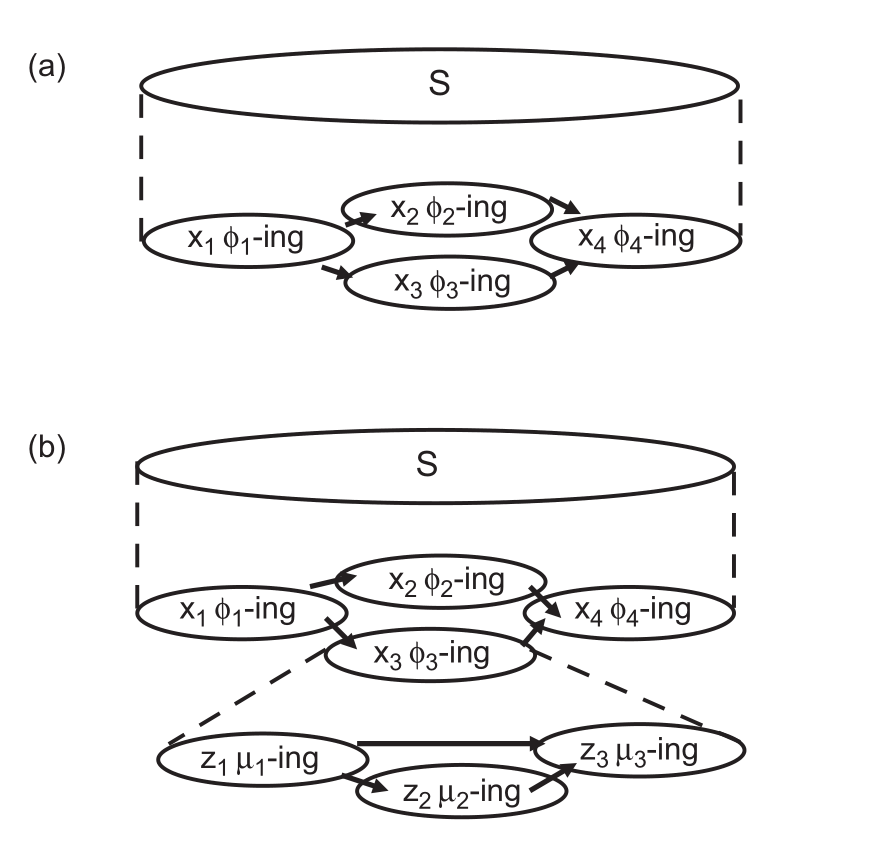
\includegraphics[scale=.3]{causalM.png}
\centering
\caption{The consensus view of mechanisms, excerpted from \cite[p.96]{Fagan2013} (a) Two levels: component x’s and overall mechanism S.
(b) Downward expansion: three mechanistic levels.}
\label{fig:CausalM}
\end{figure}

Of this view of CauMEx, Fagan writes:

\begin{longquote}
An account is “full” if and only if it describes all \textit{relevant} components of a mechanism. Causal relevance is in turn analyzed in terms of “mutual manipulability”. A working component (x $\phi$-ing) is relevant to an overall
mechanism’s behavior (S $\Psi$-ing), if the latter can be manipulated by
intervening on x's $\phi$-ing \textit{and} x $\phi$-ing can be manipulated by intervening on S $\Psi$-ing. A component is irrelevant to a mechanism if neither
x's $\phi$-ing nor S $\Psi$-ing can be manipulated by intervening on the other.
These two sufficient conditions link the hierarchical structure of MEx to
experimental practices in neuroscience, which employ both ‘top-down’
and ‘bottom-up’ strategies to detect components of mechanisms. \cite[p.100]{Fagan2013}
\end{longquote}

Therefore, we seem to have an appealing account of what biologists are doing with MEx that is neatly connected to our experimental practices. However, Fagan describes three fundamental problems with CauMEx.

\begin{enumerate}
\item  \textbf{Ambiguity}. The overall mechanism S is a causal explanation: mitosis (S) is a process of cellular reorganisation resulting in two cells being produced from the one mitosing (the phenomenon P) (Fig. \ref{fig:Ambiguity} (a)). We infer the contribution of S's components x (eg. proteins involved in spindle formation, cytoskeletal components, etc) to P by examining the effect of altering their activities $\phi$ (such as by mutating a spindle formation protein of interest) on P (Fig. \ref{fig:Ambiguity} (c)). However, usually, we take the overall explanatory bricolage we assemble of inter-component causal relations to explain S, not only P. That is, the proteins involved in spindle formation are part of a mechanism that explains the mechanism of the mitotic process itself (S $\Psi$-ing), and not only its phenomenal manifestations while $\Psi$-ing (chromosomal reorganisation, the appearance of mitotic furrows, etc.) or after S has finished $\Psi$-ing (the fact of there now being two cells).

\begin{figure}
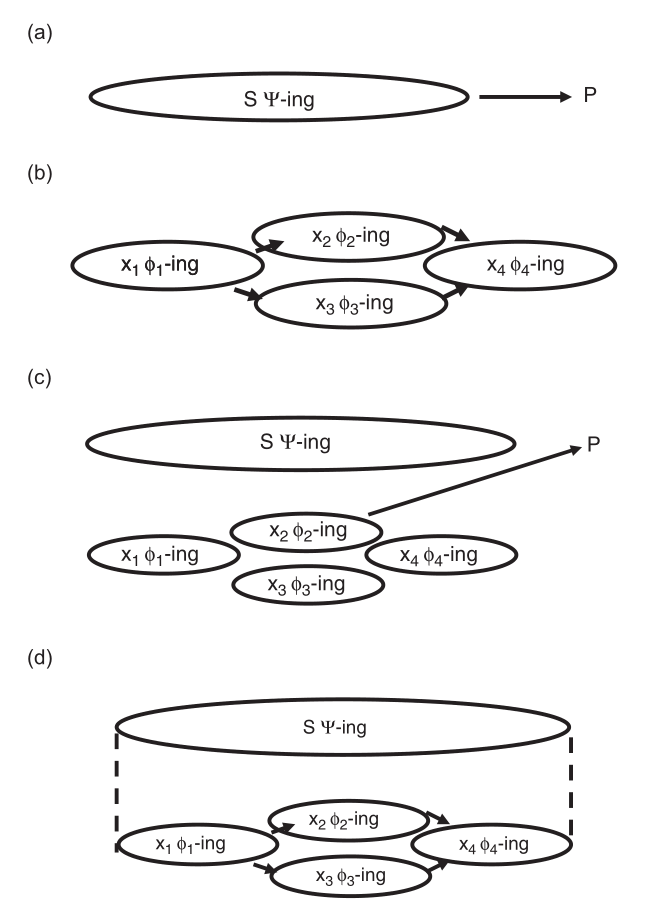
\includegraphics[scale=.5]{ambiguity}
\centering
\caption{Levels of causal relations in MEx, excerpted from \cite[p.102]{Fagan2013}.  (a) System-level: mechanism S $\Psi$-ing produces phenomenon P. (b) Component-level: component x's causally interact ($\phi$-ing) to effect one another. (c) Inter-level: component $\phi$-ing x's make a difference to S’s outcome (P). (d) Constitutive MEx: component x's interact ($\phi$-ing) to constitute mechanism S's $\Psi$-ing}
\label{fig:Ambiguity}
\end{figure}

\item \textbf{Directionality}. The assumed \textit{direction} of causal relations in the MBT is usually implied in our casual speech: we are looking for ``underlying" molecular mechanisms, which is to say, we take any ``chain" of causal relations to flow upwards from a bottom level of macromolecular components. Generally speaking, ``overarching" mechanisms in which the whole S feeds back onto its component xs in some way are not produced. Moreover, it is unclear in what sense one could impinge on the overall mechanism S and ``cause" a change in one of the components x in a ``downward" sense- as Fagan lucidly notes, intervention into a mechanism \textit{is} impinging on its components x\cite[p.103]{Fagan2013}. We are establishing a ``constitutive" relationship between S and its components x, not a causal one. This makes a nonsense of the ``mutual manipulability" interpretation of top-down and bottom-up approaches, since there is no manipulation of x by virtue of an intervention into S as a whole \footnote{As Fagan correctly notes, top-down experimental approaches are \textit{exploratory}, not \textit{explanatory}.}.

\item \textbf{Modularity}. In order for components to be defined in terms of manipulability theory, they must be independent. If we offer a mechanism consisting of generalisations about the behaviour of x$_{1,...,n}$ macromolecular processes, in order for x$_1$ to be differentiable from x$_2$, it must be in some way causally independent- we must be able to intervene into x$_1$ (eg a generalisation about DNA synthesis) without  affecting x$_2$ (eg a generalisation about membrane fusion complexes). Without some form of ``modular independence" between mechanism components, there is no reason to consider them separate, yet causally linked, ``components" of a larger overall mechanism.

However, as Fagan notes, the ``interventionist" causal paradigm implies explanations that ``reveal what a phenomenon of interest depends on, answering ‘what-if-things-had-
been-different?’ questions about the values of variables within a fixed range of invariance. But MEx are prima facie concerned with a different kind of question: ‘how-does-it-work?’" \cite[p.106]{Fagan2013} In this case, the causal relations that form ``the ways we conceptualize them as distinct, relevant components ... \textit{are the very same} causal generalizations that figure in MEx." \cite[p.106]{Fagan2013} That is, the causal relations that provide the rationale for the division of a mechanism into independent components are \textit{also} those that we take to be causing the activity of the mechanism- the components are thus not merely \textit{conceptually} but \textit{"actually", causally} separable, like components of a machine. Obviously, we understand this not to be the case. Fagan concludes:

\begin{longquote}
For physiological, cellular, and molecular mechanisms,
as we understand them, the behavior of isolated components is not a
good guide to their behavior together, and their behavior in one context
is not a good guide to their behavior in others. If this line of reasoning
is correct, then the causal-mechanical account of MEx leaves out some-
thing important: \textit{inter}dependencies among components of biological
mechanisms.
\cite[p.106]{Fagan2013}
\end{longquote}

As most modestly observant MBT benchworkers have noticed by now, components of biological mechanisms are not literally interchangeable gears that can be removed from one machine and slotted without modification into another ``geartrain" (mechanism) missing a similar component \footnote{There are a few theorists who still don't understand this, but the situation has improved. We are, now, only rarely subjected to the hallucinations of ``synthetic biologists" insisting that trees will be reprogrammed to grow chairs directly on their branches, for instance. The persistence of this fixation can be attributed to the mind-boggling success of the standardisation and modularity practices of modern logisticians, and their mechanical and electrical engineering colleagues. It is worthwhile to remember these are extremely recent developments- an artefact as modern as the Rolls Royce Merlin engine, the machine that won the Battle of Britain, did not have interchangeable parts (to the profound horror of Allison engineers in the USA tasked with setting up domestic American production of the engine). Each part was literally hand fitted for each engine by an English craftsperson. We should note that the very English metaphor for biological ``design practices" is ``tinkering" and not ``process systems engineering".}. \textit{How} x $\phi$s depends on \textit{how} it is intermeshed with other xs and what their $\phi$ing consists in. A gear only depends on the other components to the extent that it requires their presence and their intermeshing in one particular way within some tolerances\footnote{There must be at least $b$ microns of backlash for the gears to $\phi$ together (rotate mutually around their axes), or they will lock and abrade each other when the machine applies force by $\Psi$-ing, until abrasion establishes $b$ microns between them and they are free to $\phi$ or the mechanism fails (probably jammed with powdered gear teeth). Biological components ``intermesh" in a much greater diversity of ways and with far looser coupling ("slop") than mechanical ones, although every real mechanism needs a little slop in it, as the gear example indicates.} Indeed, the nature of the interdependencies between molecular components are critical to the ``how-does-it-work" explanation. As indicated in \hyperref[hierarchy]{the section on hierarchy theory}, understanding these interdependencies is especially important in ``multi-level" explanations, where xs $\phi$-ing at different dynamical scales do not \textit{directly} interact in the same manner that same-level xs $\phi$-ing do.

\end{enumerate}

Therefore, Fagan has gone on to advance what is, in my view, a much improved conception of biological MEx, the Joint MEx, to which I have made some minor additions, as described below\footnote{Fagan is an explanatory pluralist herself; in \cite{Fagan2015} she explicitly states that she does not seek to replace ``causal mechanistic" conceptions with her own JMEx. However, the conceptual problems with causal explanations she catalogues in \cite{Fagan2013} remain unresolved. If there are ``good" CauMEx, it seems to me they need a much deeper theory of \hyperref[causality]{causality} than interventionist accounts provide. For the time being, Fagan's work is adequate to stand on its own as an account of the ``local explanation" in the SCBT.}


\subsection{(Extended) Heterogenous Joint Mechanistic Explanations ((E)HJMEx)}
\label{EHJMEx}

While by ``Extended Heterogenous Joint Mechanistic Explanation" I mean a unit of theory consisting more or less of a diachronic series of Fagan's ``Joint MEx", I have a slightly different understanding of the ``explanatory components" of JMEx (jay-mex), which I have differentiated with the term HJMEx (hedge-mex). I will first clarify how I understand Fagan's JMEx improvement over the Law-based and Causal concepts. I will then define HJMEx and then explain what it means to ``extend" one for analytical purposes, producing a EHJMEx (edge-mex)\footnote{While ``fanciful" naming conventions and illegible acronyms are time-honoured traditional practices of the MBT, I apologise to readers for indulging out of a need to conserve space and stably refer to particular concepts.}.

\subsubsection{Joint MEx (JMEx)}

Fagan has described a similar improvement to the typical Causal MEx view on three occasions: first in 2012 \cite{Fagan2012a}, later in her 2013 book \cite{Fagan2013}, and most recently in a 2015 paper \cite{Fagan2015}. I have adopted the general sense of the framework described in these works, which I have called the JMEx, for Joint Mechanistic Explanation.

 Fagan's terminology varies as she emphasizes different aspects of her overall idea. \cite{Fagan2015} seems to use ``collaborative" interchangeably with ``joint," which was the preferred term in \cite{Fagan2013}. ``Collaborative" seems to be intended to emphasize the amenity of the concept to explanatory pluralism- this is one reason I have selected it, but it is less descriptive of MEx structure. I have therefore adopted the shorter ``Joint", since a commitment to explanatory pluralism \textit{within} MEx is part and parcel of the the entire foregoing description of the MBT, and respecifying it is redundant.

 Fagan indicates that both CauMEx and JMEx are species of ``Constitutive" MEx, which is to say that the mechanism consists of components that are together taken to constitute some kind of productive causal regularity which generates a phenomenon. Because a mechanism's components must be linked \textit{somehow} if they are not just to be considered separate systems, some \hyperref[causality]{theory of causality} is required to establish what these linkages might consist in. JMEx's account of ``intermeshing properties" is sufficiently general that MBT practitioners with different ideas about causality can talk to each other about these properties without needing to carefully specify either a particular local causal account with significant problems (manipulability theory) or a fully worked-out global theory of causality.

Fagan's solution to the problems with Causal MEx dispenses with the problems her analysis of them revealed. Let us recapitulate Fagan's formulation of Causal MEx (M) and follow it with her JMEx formulation (JM) for comparison\footnote{\label{ftn:JMedits}I have used \cite{Fagan2015} (JM) as it contains the \cite{Fagan2013} definition but is more precisely worded. I have changed ``system M" to ``mechanism S" to conform with the other citations of \cite{Fagan2013} used here, but this does not change the meaning in any way.}.

\begin{longquote}
(M) A mechanism S consists of multiple diverse components (x's) engaging in causal relations or activities ($\phi$'s) such that x's and $\phi$'s are 
spatially and temporally organized so as to produce some overall
phenomenon.
\cite[p.95]{Fagan2013}
\end{longquote}

\begin{longquote}
(JM) Components x$_1$,\ldots x$_n$ jointly $\Psi$ as mechanism S if and only if


(i) each x$_i$ has properties that mesh with one or more other x$_i$,

(ii) x$_1$,\ldots x$_n$ are spatially organized and their activities $\phi_1$-ing, \ldots $\phi_m$-ing causally organized in virtue of their meshing
properties,

(iii) x$_1$,\ldots x$_n$ and $\phi_1$, \ldots $\phi_m$ so organized constitute mechanism S $\Psi$-ing, and

(iv) x$_1$,\ldots x$_n$ and $\phi_1$, \ldots $\phi_m$ not so organized do not constitute S $\Psi$-ing

[See footnote \ref{ftn:JMedits} for description of clarity edit made to (JM)]
\cite{Fagan2015}
\end{longquote}

Fagan elaborates on what would therefore constitute a good JMEx:

\begin{longquote}
(JM) suggests a basic norm for what I shall term 'collaborative
explanation,' namely, that a successful explanation of this kind must
show that the components and system of interest (the target of the
model) satisfy the conditions of (JM). Given a set of components and
their associated activities, and an overall system exhibiting some
behavior, an explanatory model of the latter should describe:

(i) the properties of components that allow them to interact in
specific ways (I.e., meshing properties, as well as other conditions, such as spatio-temporal proximity.)

(ii) the spatial and causal organization determined by these
interactions

(iii) how the overall system behavior is constituted by the
organized components, such that

(iv) components' organization makes a difference to the overall
system behavior.

[I have expanded Fagan's footnote related to item (i) as a parenthetical comment]
\cite{Fagan2015}
\end{longquote}

This strikes me as an entirely adequate definition for MEx, as well as a prescriptive norm for ``good" or ``complete" explanations that provides a reasonable broad guide to what sort of things MEx should eventually be able to do for the system they explain. Moreover, with JMEx, Fagan resolves all three problems with CauMEx simply by replacing manipulability theory with her conception of Joint relations between MEx components, which I find a highly convincing demonstration of the conceptual adequacy of Jointness.

\begin{enumerate}
\item \textbf{Ambiguity} is resolved. The component xs of JMEx are understood to be interdependent and linked by descriptions of their intermeshing properties expressed while $\phi$-ing (eg. binding, activation, phosphorylation, and so on). It is the assemblage of xs, linked by virtue of these properties, that constitute mechanism S $\Psi$-ing, so that we are explaining this overall activity of S with our JMEx, which in turn is understood to produce P.

\item \textbf{Directionality} is clarified. JMEx ``bottom out" at the level of macromolecules, in general, and do not typically reference ``lower levels" in the scale hierarchy, like atomic or electronic phenomena. We understand that when we intervene experimentally into the activity of some system S that a mechanism describes, we are not having a ``downward" effect on the mechanism's components x in their $\phi$-ing, but that intervening into S \textit{constitutes} intervening into some x, all the way down levels of organisation to the MBT's ``explanatory foundation" macromolecular level.

\item \textbf{Modularity} is dispensed with. Given the ``Jointness" account of the intermeshing properties of components x of JMEx, he rationale for their ``separateness" does not depend on manipulability theory. Therefore, we are able to account for the interdependency of the mechanism's components and avoid implying that we believe we can intervene into one component in a manner that causally isolates it from the others.
\end{enumerate}

Having summarised Fagan's JMEx concept and its fine qualities, let me pause to point out an interesting feature of JMEx: the ``jointness" or ``collaborative" account of causal relationships between JMEx components is adapted from social scientific accounts of \textit{shared cooperative activity} (SCA), that is, the intentional, end-direct activity of multiple agents collaborating. As Fagan indicates, her analysis of joint activities ``is modeled on (Bratman 1999)[\cite[pp.93-108]{Bratman1999}], with adjustments for non-intentional contexts." \cite{Fagan2015} I return to some aspects of Bratman's description of inter-human SCA for useful \hyperref[agentmodel]{ideas about agency later}, but overall, Fagan's adjustments make perfect sense. She has chosen to ``strip down" an account of joint action between people in order to produce one that fits, say, signalling pathways, which clearly have no psychological states, and of which it is meaningless to speak of ``intent". Moreover, the ``stripping down" leaves an excellent skeleton which can be ``refit" in a conservative, non-psychologising manner that admits \hyperref[biosemiotics]{biosemiotic} descriptions of cellular agents, at the appropriate levels and with regard to the appropriate ``meshing properties". 

This makes JMEx a spectacularly good type of explanation for multi-level mechanisms that incorporate \hyperref[agentmodel]{\textit{bona fide semantic agents}} like cells. We expect to be able to express JMEx for higher-level phenomena like tissue formation because we can plausibly represent the joint, coordinated activity of the cells that constitute the tissue as agents.

I take a substantially different view of how ``systems biology" is related to JMEx, however, which I have explained below. Firstly, while Fagan is clearly a sophisticated philosopher of biology, and a masterful documenter of the ``local model terrain" in the SCBT, her particular vision of JMEx that has a two limitations for my purposes. I have addressed each limitation in turn, in the context of my proposed solutions: the ``H" and the ``E" (proceeding outward from the core JMEx concept) of the EHJMEx.

\subsubsection{Heterogenous JMEx (HJMEx)}

 The first of these limitations to JMEx, as presented by Fagan, is related to an epistemological and metaphysical stance shared with the influential master historian of the MBT Evelyn Fox Keller, who offered her own thumbnail sketch of the \hyperref[SBE]{SBE} some 18 years ago:

 
\begin{longquote}
"Out of the wickedness of war," wrote Warren Weaver in
1949, in a paper entitled ``Problems of Organized Complexity," ``have come two new developments \ldots of major importance in helping science to solve these complex twentieth-century problems." The first of these was the electronic
computer, built to process the masses of data generated
by the procedures of modern warfare—and, perhaps most
famously, to decipher enemy messages encoded in ever
more elaborate encryption devices. The second development is most commonly associated with the word \textit{cybernetics}, Norbert Wiener's term for the study of control and communication in machines and living beings. Extrapolating
from his experience with ``goal-oriented" and ``self-steering"
devices designed to improve the accuracy of anti-aircraft artillery, Wiener and his followers envisioned the construction
of purposive machines that would resemble living organisms in every way. Indeed, these machines would be built on
the very principles of circular causality ("in which every part
is reciprocally both end and means") that Kant himself had
invoked as the defining feature of the organism.

These two developments were clearly related-at the very
least, they were related in time, in place, and in the needs
from which they arose. Yet despite their persistent conjoining in the popular imagination, despite Wiener's own
hopes, and despite even John von Neumann's efforts at integration, conspicuous differences between the two remained.
In the one the emphasis was on computational power, while
in the other it was on principles of organization and—increasingly over the 1950s and 1960s—of self-organization. 
In fact, in was not until the 1980s that the different visions
embodied in these two developments would begin to resolve, and the first steps of that resolution came with the
rise of connectionism, parallel processors, and neural networks. Yet Jacob’s claim that the sequence of DNA could
serve as Bernard’s ``invisible guide" depended absolutely on
joining together these two still-disparate developments. His
metaphor of a program drew directly from Turing’s original
model of a computer (the reader may recall from Chapter 1
his equation of ``the genetic material with the magnetic tape
of a computer"), but the idea of a purposive machine was
borrowed from Wiener's cybernetic vision. The difficulty is
that, in locating the program in the genome, much of the
cybernetic vision of goal-seeking and self-organization was
lost. And so was the recognition of the importance of reliability and with it, an appreciation of the kinds of organizing principles that would be needed to maintain such reliability. Redundancy, for example, is a basic principle of
design for building reliable systems, and it is hard to imagine how, were it not for this amnesia, recent findings of extensive redundancy in developmental pathways could have been quite as startling as they have been.
\cite[p.109-111]{Keller2000}
\end{longquote}

That is, on Keller's view, the ``molecular reductionist" trend in the MBT, myopically fixated on Crickian information flow outward from genomes, lost sight of the need to deploy the fruits of the IT revolution and of cybernetic theory to explain ``goal-seeking" and ``self-organisation", which is to say, agency. The logical solution to this quandary is to do precisely what Fagan suggests- reintroduce the \hyperref[cybernetics]{\textit{cybernetic formula}}, levering the computational power of modern semiconductor devices to solve systems of ordinary differential equations (SODEs), treating cells as a type of complex chemical system with Dynamical Systems Theory (DST). Both Keller and Fagan believe this is a reasonable way to find the macromolecular basis for \hyperref[Waddington]{Waddington's classic theory} of cellular specification. Fagan makes this view explicit in her definition of mathematical ``Systems" approches to JMEx:
 
\begin{longquote}
A cellular systems model consists of a finite set of molecular elements
$\{X_1, X_2 … X_n \}$, representing DNA, RNA, proteins, and small molecules.
Complexes of multiple components and functionally-distinct forms of
one molecule are represented as distinct, so the set may be larger than
a simple parts list. Each molecular element in the set is characterized by
a value of a state variable $\{x_1 , x_2 \ldots x_n\}$ at time $t$. In these models, the cell
is defined as a complex system which at any time $t$ is in a state $S(t)$ that
is fully determined by the values of a set of variables $\{$x$_1$, x$_2$ \ldots x$_n \}$ representing the state of each molecular component. The values of these
variables exhibit numerous and diverse dependency relationships. Cell
behavior, including development, is conceived as the result of changes in
the values of state variables. A set of molecular elements, each described
by a state variable, and dependency relations between the values of those
variables, comprises a cell network model.

In this way, systems biologists aim to derive predictions about cell
behavior, including developmental phenomena, from mathematical
descriptions of interacting molecules. Insofar as these predictions are
confirmed by experiments, the mathematical models that entail them
can be said to explain the phenomena in question. The process of model
construction begins with detailed description of a molecular mechanism.
This mechanistic description is then simplified into a wiring diagram,
which is next translated into a formal framework. Solutions within a
formal framework correspond to vectors and attractors, and these vectors
and attractors in turn define a 'landscape.'
\cite[p.204]{Fagan2013}
\end{longquote}

Fagan has advanced this prescriptive view of what Systems biological approaches to JMEx consist in on several occasions, so that she has produced a useful summary diagram, reproduced in Figure \ref{fig:faganSystems}. The most obvious feature of the diagram for the student familiar with MBT models is its linearity: there is \textit{only one} Systems approach represented here.

\begin{wrapfigure}{l}{0.4\textwidth}
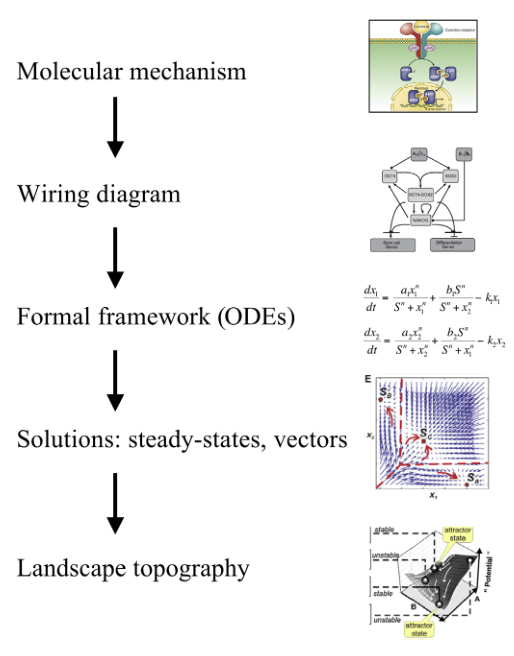
\includegraphics[scale=.36]{Fagansystems}
\caption{Cellular systems model-construction, excerpted from \cite[p.7]{Fagan2015}. The system of equations and subsequent steps are based on a 2-element wiring diagram.}
\label{fig:faganSystems}
\end{wrapfigure}

While most MBT practitioners and students are familiar with this approach, what is most notable about it is that it is, in practice, rarely applied in this form. Part of the reason for this is technical problems in relating complex macromolecular systems to formal SODEs, which I have summarised in the section \hyperref[SODEs]{relating to that method} and its theoretical underpinnings. In general, however, I have gone against this ``Systems formalisation scheme" for the following reasons:

\begin{enumerate}
\item \textbf{Actually Existing MEx Pluralism}. Harris' theory, like most others, does not use DST to produce topographies that represent some kind of ``Waddington space". While much effort has gone into DST-type formalisations of mechanisms, there are other types of ``Systems explanations" that must be accounted for.

\item \textbf{Unclear General Utility}. While SODEs offers a plausible formalisation of \hyperref[Waddington]{Waddington's view}, it is not at all clear that all or most cellular processes involve transitions between attractors in some state space whose dimensions express protein expression levels or estimates of activity. Waddington's view of the cell is of a probability landscape of \textit{chemical tendencies} extended in time, underpinned by genes and the interactions of their products (see Fig. \ref{fig:Waddington}). This is the conceptual conceit that allows macromolecular relations to be treated as a system of ODEs; their interactions are understood ordered chemical reactions in cellular ``bioreactors". I see no reason to presume that this is an adequate modelling frame to explain phenomena where, for instance, the specifics of local inter- and intracellular spatial organisation is as or more salient than chemical kinetics, as in many emerging MEx related to nuclear behaviours, transcription factories, tissue formation, etc. 

\item \textbf{Commitment to Open Exchange}. As noted in Section \ref{open}, I am taking some care not to dictate what post-Systems biology ought to look like. I do not know what ``systems" disciplines will ultimately prove to be successfully integrable into the MBT. Given the potential of, for instance, \hyperref[physex]{physical explanations} to contribute as components of MEx \cite{Morange2011} or of limits on them, it seems unwise to exclude these by adopting a MEx concept that does not allow for their inclusion, or of other methods that may prove useful. I am in particular concerned with the formation of subtraditions committed to particular mathematical approaches and not able to meaningfully compare their model formalisations.
\end{enumerate}

I have, instead, treated ``Systems" approaches as methods of generating extra-traditional generalisations about the components of mechanisms, so that a ``Systems" JMEx does not necessarily summarize the activity of the entire mechanism (S $\Psi$-ing) using one particular mathematical method, but may draw from any number of traditions in generalising about x's $\phi$-ing.

There are at least two concerns with this sort of ad hoc modification: the possible loss of biological macromolecules as the lowest level of organisation represented in MEx, and the possible loss of the multi-level logical relations constituting the ``Joint action" of macromolecular x's $\phi$-ing together to constitute an S $\Psi$-ing. I address these in turn:

\paragraph{HJMEx may specify their ``bottom" macromolecular levels polysemously}\mbox{}\\
 Firstly, Fagan's JMEx concept usefully explains the fact that MBT explanations tend to ``bottom out" at the macromolecular level. This is generally recognised and is often offered as a reason for considering the MBT to be meaningfully independent from physical and chemical traditions. We rarely make reference to physico-chemical properties of biological molecules, except in defining their activity ($\phi$-ing) or their relations (how x$_1$ jointly $\phi$s with x$_2$'s $\phi$-ing). I do not want to lose this feature of Fagan's JMEx. 
 
 At the same time, we often offer generalisations about molecular behaviours that we intend \textit{polysemously}. Let us take the example Fagan offers of the mechanism for \textit{Drosophila} germ stem cell (GSC) specification- as Fagan notes, most (80\%) but not all mitoses proceed by employing this mechanism. However, if we want to model the cellular population dynamics of a whole \textit{Drosophila} embryo, we probably will offer a generalisation about a mitosis as a \textit{process}- that is, we are interested in the \textit{total number of divisions}, irrespective of their molecular mechanisms. If we were interested in (a)symmetric divisions, we would actually want to specify something like Kitcher's \hyperref[PS]{PS-process} concept, which could conceivably be accomplished by any number of mechanisms. Therefore, a JMEx that made reference to ``mitoses" in general, or ``symmetric" divisions in particular, could well have a description of some x that $\phi$s on a higher-than-molecular level of organisation, that does not reduce directly to any particular set of molecular zs $\mu$-ing, to use the terminology of Fig. \ref{fig:CausalM}. Instead, it may refer to any number of MEx, and is thus ``polysemous" in the sense that it is constituted by more than one entity at the ``macromolecular basement" level\footnote{This polysemy essentially specifies all actually-present mechanisms S that $\Psi$ such that some P occurs. It is very likely that eg. mitosis, in most contexts, is driven by a smaller number of mechanisms that account for a majority of divisions, but a very large number of mechanisms that account for rare ones (these could even be completely unique). If we are accounting for cell number in a tissue, we do not care if a mitosis was produced by a miraculous, unique mechanistic causal locus or not. A division is a division.}  One could conceivably add more detail ``below" this level if necessary, but in general, there is every reason to expect MEx to have components that are not usefully broken down beyond a certain level, and which, when applied in an abstract or theoretical manner, may not even refer to stable molecular entities at all\footnote{Arguably, a PS-process is a basic requirement for a living thing, defined as a replicating semiotic agent. Semiosis implies an interior and an exterior, so a membrane or wall of some kind, forming a cell. ``Replication" in the strict sense must then proceed by duplication of the agent's contents and segregation by dividing its contents into two membrane compartments. To the extent that the selection of macromolecular materials used in living systems is historically contingent, there will be a correspondingly large number of possible material substrates and intermeshing properties that produce such a process.}.
 
 However, as I hope is clear, I do not mean to imply that a CGT traditional concept like a PS-process has some reality \textit{independent} of the specific macromolecular arrangements that actually constitute cells dividing and partitioning their contents between two descendants. The fact that the CGT concept does not reduce cleanly to a set of one or more MGT descriptions of macromolecular processes in nuclei may or may not be relevant to the explanatory quality of the JMEx which uses the CGT concept as a stand-in for many different MGT-specifiable cellular dynamics. To a large extent, this depends on what we suppose the intermeshing properties of the mitotic process and the other components of the mechanism to be. That is, if we suppose mitosis (call it x$_1$ $\phi_1$-ing) to be mainly independent from other relevant cellular behaviours we are modelling (x$_{2\ldots n}$ $\phi_{2\ldots n}$-ing), it may not matter whether we have any account of the specific macromolecular arrangements (z$_{1\ldots n}$ $\mu_{1\ldots n}$-ing together), which we take to constitute x$_1$'s activity, to expand our HJMEx ``downward".
 
 Moreover, we understand that any time we propose an experiment which intervenes onto some x $\phi$-ing, where the HJMEx uses a polysemous generalisation including many macromolecular arrangements of zs $\mu$-ing jointly, that intervention is onto some subset of actually-occurring, specifiable-in-their-particulars macromolecular z$_{1 \ldots n}$ and  $\mu_{1 \ldots n}$-ing together. That is, the use of polysemous generalisations in no way implies that an intervention is not ``directly" onto the macromolecular materials constituting an organism. For example, if there is more than one macromolecular process which produces mitosis in some cultured cells, and we apply a chemical inhibitor of mitosis, we understand that we are going to intervene into that polysemous distribution of possible macromolecular developments that result in mitosis. Which mechanisms are actually affected depends on how common those macromolecular trajectories\footnote{I mean this in the loosest possible, non-Newtonian, non-quantitative, non-state space sense.} are and how the chemical inhibitor affects the components and intermeshing properties of each one. Chemical inhibitors of mitosis that broadly affect commonly used mechanisms would be promiscuous inhibitors of a macromolecularly polysemous behaviour, validly described by polysemous CGT generalisations about mitosis. We may be interested in specific inhibitors if they are available, but inhibitors of rarely employed mechanisms will probably never be discovered in the first place, due to the population-based assays typically used in drug discovery.
 
  Conceivably, this could lead to a class of MBT HJMEx that are composed entirely of generalisations which cannot be reduced to particular biological macromolecular relations at all. This seems like a plausible outcome of the SBE- a class of models that deal exclusively with phenomena at higher levels of biological organisation, polysemously referring to huge arrays of unspecified molecular arrangements (perhaps consisting of statistical generalisations about assemblages of possible mechanisms S that $\Psi$ to produce P). It seems very unlikely to me that these will be anything more than toy models and curiousities without strong grounding in the MBT's foundational explanatory level, however, so this does not seem like a likely risk to MBT \hyperref[stability]{traditional stability}.   
 
 \paragraph{HJMEx retain constitutional directionality and allow causal nuance}\mbox{}\\
 
 The second potential problem involves the potential confusion involved in incorporating extra-MBT causal generalisations at higher levels of biological organisation. For instance, there is much interest in tension and shear-induced signal transduction involved in morphogenesis \cite[p.5]{Malagon2015} as contributors to \hyperref[emergence]{self-organisation} and biological complexity. Therefore, HJMEx might include \hyperref[physex]{physical explanations} at very high levels of organisation. It is unclear that all such explanations can be understood to proceed from the ``bottom up".
 
 Let us take one such HJMEx that already circulates ``in the wild": behavioural impingement on osteoblast development and bone dynamics. Bone, being a highly dynamic tissue, actively remodelled in response to stress, has structural and functional aspects that are determined by organismal behaviour, psychological states, etc. This is obvious when we consider what we have to do to ``model" the effects of microgravity conditions on bone dynamics in rodents: the hindlimb elevation assay (HEA?), ie. restraining the animal such that its organised behaviour cannot create normal stresses on the bone, which in turn results in bone mineral density loss\footnote{I have placed ``model" in scarequotes because it is not at all clear to me that you can study the effects of microgravity except in a 1g laboratory. Microgravity-related BMD loss being a behavioural disease of a tiny number of humans (astronauts), taking on this risk with full informed consent, it is hard to see how it can be ethical to torture thousands of rats with these assays in order to ``study" this ``medical issue".}. This occurs via the sensing of tissue-level strain by osteocytes, which in turn direct the action of osteoblasts and osteoclasts\footnote{Osteoblasts lay down bone, osteoclasts destroy it. The local balance of osteoblast/clast activity determines whether bone is plated out or broken down at a given site.} in remodelling the overall structure of the bone to better suit the actually-experienced load.

 A component of a HJMEx describing bone remodelling might therefore include a statistical generalisation of behaviourally-conditioned bone stress dynamics (say, a finite element analysis of a rat's bone under normal behavioural strain over some period of time). It is not immediately clear how such a HJMEx should be hierarchically arranged. Conceivably, a description of the rat behaving could be a ``mechanistic" system S $\Psi$-ing, which includes the details of the molecular mechanisms underlaying osteocyte strain sensing as low-level zs $\mu$-ing in mainly-macromolecular MEx. This ambiguity leaves space for those with \hyperref[causality]{directional theories of causation} to claim that one may intervene onto the rat behaving (S $\Psi$-ing) and so cause a downward cascade through mechanistic levels and ultimately impinge onto the basement level in this manner, implying a similar problem to the one we identified with the mutual manipulability account of MEx.
 
 I respond to this in two ways:
 
\begin{enumerate}
 
\item Firstly, HJMEx retain ``constitutional" directionality in two senses:

(a) there is a ``basement" level but no ``ceiling" ("sky's the limit", organisationally). That is, HJMEx assume that the biological scale hierarchy \textit{necessarily starts} at the level of molecular biological material \textit{simplicter} and proceeds upwards through macromolecular assemblages, organelles, organelle lineages, cells, cell lineages, tissues, organisms, organismal lineages, local ecosystems, planetary ecosystems, and then, hypothetically, interplanetary ecosystems, intersolar ecosystems, and so on\footnote{Theories of panspermia typically postulate intersolar ecosystems with planetary ecosystem components connected by their ``intermeshing property"- their propensity to fling debris into space under the impact of asteroids, etc.}.

(b) HJMEx imply that interventions at higher levels \textit{constitute} intervening at the lowest level. If humanity intentionally destroys the planetary ecosystem by raising the average temperature of the planet to the point where plants no longer reliably germinate, this \textit{is} an intervention at the lowest possible biological level of organisation of all organisms. Unloading the rat's limbs \textit{is} intervening onto macromolecular processes in osteocytes.

 This is completely sufficient for understanding the structure of a causal locus as I have defined it, and it retains JMEx's accurate reflection of the ``bottoming out" of biological MEx at the macromolecular level.

 \item Secondly, HJMEx deemphasize simplistic ``directional" accounts in favour of detailed exploration of the intermeshing properties of JMEx at different levels of organisation.
 
 Let us again take up the example of osteoclast strain sensing. There is a significant problem in the potential representation of a Mechanical Engineering Tradition (MET) finite element analysis (FEA) as a generalisation of the effects of rat behaviour on bone loading. The FEA is a description of the physical dynamics of tissue, measured on a spatial scale of (perhaps) millimeters, and a temporal scale of seconds. Now, macromolecular dynamics occur on spatial scales of nanometers and temporal scales of microseconds! There is therefore a dynamical barrier in this scale hierarchy, discussed further in \hyperref[hierarchy]{the section on hierarchy theory}.
 
 What is interesting to us then is not a question of causal priority or ``directionality" but a question of ``how-does-it-work", a request to elucidate the intermeshing properties between the extra-traditional MET FEA and whatever model we have for macromolecular osteoclast strain sensors. The interesting question is \textit{how} information about strain is brought across the dynamical barrier by the strain sensor, and \textit{how} the resultant activities of osteocytes, osteoblasts, and osteoclasts act to alter the bone's structure such that its stress/strain properties evolve under load.
\end{enumerate}
 
Therefore, HJMEx allow us to accurately represent contemporary ``Systems" theories, while retaining the MBT's understanding of the explanatory ``macromolecular basement". By emphasizing the intermeshing properties of mechanisms, and their part-whole relations, we can move past problematic causal generalisations into specific descriptions of these properties.

\paragraph{HJMEx defined}

Fortunately, little needs to be done to Fagan's JMEx (JM) definition to differentiate HJMEx. I have indicated these clarifications with HJM-n notations.

\begin{longquote}

(HJM) Components x$_1$,\ldots x$_n$ jointly $\Psi$ as mechanism S if and only if

(i) each x$_i$ has properties that mesh with one or more other x$_i$,

(ii) x$_1$,\ldots x$_n$ are spatially organized and their activities $\phi_1$-ing, \ldots $\phi_m$-ing causally organized in virtue of their meshing
properties,

(iii) x$_1$,\ldots x$_n$ and $\phi_1$, \ldots $\phi_m$ so organized constitute mechanism S $\Psi$-ing, and

(iv) x$_1$,\ldots x$_n$ and $\phi_1$, \ldots $\phi_m$ not so organized do not constitute S $\Psi$-ing

HJM-1: Each x$_i$ $\phi_i$-ing consists of a description of the behaviour of a biological system at the macromolecular level of organisation or higher.

HJM-2: At any level of organisation higher than the macromolecular ``basement", each x$_i$ $\phi_i$-ing may describe one or more lower level mechanisms S $\Psi$-ing polysemously, and need not specify any of these S in any particulars.

HJM-3: Polysemous xs $\phi$-ing describe general properties of a population of Ss $\Psi$-ing that intermesh with other xs $\phi$-ing, and these need not arise as a consequence of specifically defined macromolecular mechanisms S.

HJM-4: Polysemous xs $\phi$-ing may have general properties that intermesh with zs $\mu$-ing on lower level, such that there is an interlevel exchange of information (boundary conditions are placed on an assemblage of zs $\mu$-ing, for instance), and these need not arise as a consequence of specifically defined macromolecular mechanisms S.

HJM-5: All descriptions x are drawn from some scientific tradition, and so carry with their use an array of traditional natural assumptions, epistemological and metaphysical axioms, methodological considerations, and so on. No x is \textit{a priori} excluded from inclusion in HJMEx on the basis of its traditional identification alone.

\end{longquote}

HJMEx are therefore somewhat more complex than JMEx, and require careful attention to the physical and biological plausibility of between-component and interlevel relations. That said,the ``basic norm" that Fagan suggests for JMEx is upheld for HJMEx. Good HJMEx describe (i) the properties of components that allow them to interact in specific ways, (ii) the spatiotemporal-\textit{cum}-causal organisation produced by these interactions, (iii) the sense in which the overall system's behaviour is constituted by the components, (iv) in a manner that explains how the organisation of components makes a difference to the system's behaviour.

 Having so-defined HJMEx, let us proceed to consider how we might assess the development and deployment of these explanations in scientific research programs.

\subsubsection{Extended HJMEx (EHJMEx)}

I have further modified the HJMEx concept by suggesting extending it in time over its career, iteratively deployed as an explanation in different studies. I have taken this idea from Kenneth Schaffner's idea of the ``Extended Theory". As Schaffner says of his own ``metascientific unit":

\begin{longquote}

I am using the notion of an \textit{extended theory} to introduce a diachronic unit that (1) permits \textit{temporal} theory change and (2) also allows for some \textit{logical} changes - namely, some of the assumptions within the diachronic unit will change while the integrity of the whole is preserved. 
\cite[p,211]{Schaffner1993}
\end{longquote}

 Schaffner was working with a substantially different conception of a biological theory\footnote{In effect, Schaffner wanted to be able to compare Lakatosan ``research programmes" consisting of lawlike generalisations arranged in hierarchies of centrality to the overall programme.}, but my intent is similar. There are numerous reasons to describe a theory's development in time. I have done so because I was unable to assess, by inspection, the broader significance of changes to components of the theory as expressed in different primary reports over time. 
 
 By representing a changing HJMEx over time diagramatically, I am able to better understand the relationship of changing theoretical structure to the model output and explanatory power, since I can compare the output of different HJMEx to empirical data in the \hyperref[model] {global model selection approach}. Moreover, this diachronic approach provides insight into the dynamics of a particular theoretical construct over time, so that we can form an idea of whether a given EJMEx is becoming more or less useful, consistent, precise, etc., and possible reasons for this.
 
 \paragraph{EHJMEx defined}

 There is little additional nuance to EHJMEx, so let us simply define one as a series of HJMEx explanations, arranged in chronological order, such that the EHJMEx reveals the diachronic explanatory dynamics of the changing HJMEx being offered by a particular research program\footnote{One might also conceive of a complex HJMEx phylogeny, branching as different researchers adapt the HJMEx for their own local purposes, rather than a linear sequence.}. I suggest that presentations of EHJMEx would normally be marked up in such a way that the changing components of the explanation and the relevant traditional implications are highlighted.

\section{The Feyerabendian Modeller}
\label{model}


If we understand the value of the interaction of scientific traditions in Feyerabendian terms, we become sensitive to the metaphysical contrasts induced by when we cognitively compare explanations produced by two or more traditions. A valid contrast between traditional explanatory frames occurs when we come to correctly understand \textit{how} the two traditions' metaphysical implications differ\footnote{Invalid metaphysical contrasts can be drawn, as from misunderstanding or malice, and there may even be rhetorical sleights of hand that make these errors seem consistent, so one must be alert during this process. Biologists are better aware than anyone of how easy it is to ``fool oneself", hence our attachment to blinding procedures.}. If we are pursue this as a deliberate practice, particularly with the regard to the details of (E)HJMEx, it would be helpful to have a systematic way of making these contrasts. It is difficult to cognitively explore the full implications of some outside-MBT ``Systems" artefact, like a solution to a system of ODEs, without an equally systematic exploration of the implication of that explanation \textit{and its alternatives} for the phenomenon at hand.

Therefore, we are interested in an approach that can reveal the \textit{systematic implications} of arbitrary HJMEx for the dynamics of our system. By this, I mean we want to make formal comparisons between model output for some group of proposed HJMEx, with to their explanatory power for some set of real data. We would also like to ensure that the approach is sufficiently general that it can be used to generate comparable output for HJMEx irrespective of the traditional or methodological makeup of their ``explanatory components". In other words, if someone comes to us with a verbal description of rules that a retinal progenitor cell might follow on its morphogenetic trajectory towards integrating into the neural retina, this should be comparable to any complicated set of statistical generalisations about the same kinds of cellular behaviours.
\subsection{Laws, Rules, Models, and Games}
As should be clear from our foregoing discussion, we are not expecting to encounter enough ``laws" in HJMEx to describe the overall explanation as ``Law-based". Nonetheless, one obvious consequence of admitting physical explanations into JMEx is that we may encounter traditional claims which include ostensible \textit{bona fide} laws\footnote{Various traditions may also posit a priori logical or reasoned truths. We tend to agree that typical logical syllogisms do not need justification, but we rarely examine the logical background of our claims (why are they justified? what is their structure?). The science of logic seems underutilised in the biological sciences.}, alongside our typical diagramatic macromolecular JMEx. These may be integrated into explanations that involve something like verbally conveyed heuristic rules ("no differentiation for the first 2 rounds of mitosis"), as well as sophisticated mathematical simulations of phenomena, or statistical generalisations about higher-level phenomena (ie. ``mathematical models" in general) whose molecular underpinnings are unknown or not relevant.

There tends to be some ambiguity in the way that we use these terms, and a necessary anthropomorphic projection onto a phenomenal reality of transcendent complexity and informational density. If by ``law" we mean that the mathematical description of some natural regularity offered by one of the physical subtraditions is \textit{actually existentiated} as some kind of iron fisted algorithmic tyrant, we have a very strange sort of ontology\footnote{Richard Swenson has memorably described the definition of genes and memes as ``selfish", Ideal algorithmic replicators (which cannot be the case, as neither is a valid unit of selection) as a form of ``Neopythagorean Reductionism".\cite{Swenson1997}. This sort of covert Idealism is a byproduct of the unresolved Cartesian fissure mentioned in the discussion of the \hyperref[SBE]{SBE}. It is, ironically (since advanced by militant atheists), the product of Descartes' bifurcated \textit{Christian} ontology. Unable to fully digest Greek philosophy properly rooted within its Abrahamic heritage, the Greek Pauline church was unable to confer upon its Catholic and Protestant progeny a viable monist ontology capable of providing a reasoned approach to study of causal regularity in phenomenal reality, and was forced to divide existence between the fallen ``natural" world and an infinitely transcendent ``supernatural" plane, interacting indirectly through providence (the workings of which were irretrievably compromised by the identification of First Cause with a particular human being). It was inevitable that this divide would be reproduced in Rene Descartes' ontology as ``matter" and ``mind", and thenceforth to the absurd spectacle of ``scientists" denying the reality of their own minds while covertly presupposing an invisible mathematical realm where algorithms vie for dominance.} We know, of course, that our physical descriptions of the world are also ``models", that Newton's Laws are not God's Laws, nor Nature's Laws, but a set of finely honed mathematical approximations of macroscopic mechanical phenomena local to a particular gravity well. We do not speak of Quantum Laws but of Quantum Theories, of the Standard Model of physics, and so on. We should nevertheless be clear that no reasonable person any longer believes that there is a ``true model", a generative algorithm ``actually out there", that can be discovered by comparing different candidate formulations until the ``correct" one is found, thus settling the issue of what the ``true" set of laws, set of rules, model, or whatever ``actually" is. Systematised knowledge about phenomenal reality is \textit{made possible} by abstracting away from the unique momentary particulars of each example of some general class, and any type of theory or model involves abstractions. That is to say, any biological explanation is by necessity \textit{not} a complete recapitulation of the system that generated the original phenomenon.

In this thesis I have, for the most part, described EHJMEx as ``explanatory programs" or ``bodies of theory", HJMEx as ``explanations" or ``theories", and reserved the term ``model" for particular mathematical formalisations used either (a) as components of HJMEx ("component model") or (b) as summaries of the overall output of HJMEx ("summary model") for some parameters of interest. I am not very interested in enshrining any of the diverse components of HJMEx or the explanations themselves as ``laws", but we can usefully speak of ``rules" that connect them- the intermeshing properties of various HJMEx components will often be simple prose descriptions of how one depends on the other. These ``rules" are more like human-generated legislation than Divinely-\textit{cum}-Naturally ordained Law- we do not expect cells to always and everywhere ``follow the law", subject to a tyrannical deity or algorithm. They will, of course, break some of any conceivable set of rules if one observes enough cells long enough.

 I therefore suggest that we think of HJMEx in this context as a the ``rules" to a type of simulated game. This is appropriate, given that systematic Western modelling of complex biological phenomena has deep roots in the evolution of games like Kriegspiel. Indeed, the widely-known toy Conway's ``Game of Life" is a type of cellular automaton closely related to the spatially-situated NetLogo models employed in this thesis. Biologists are thus generally familiar with this type of simulative ``game". In comparing summary models of our explanations, we are not asking ``which of these models is actually true", but ``which of these games is most 'realistic'". We mean something more quantitative than this, of course, which is related to information theoretical measures of information loss between empirical reality and model, as discussed below. It is, nevertheless, necessary to differentiate between the \textit{rules} of the ``game" (the overall HJMEx offered in some publication), the \textit{specific interpretation} of the rules that gives rise to the actual implementation of the game (eg. the procedural logic of some summary model that we use to elucidate what the HJMEx ``game" implies about the system it represents)\footnote{Any set of rules requires an interpreter who implements them. Particularly annoying and tendentious interpreters of game ``rules" are often called ``rules lawyers", and the same sort of hermeneutic or interpretative activity is always present when confronting the necessary ambiguities in a ruleset. Generally speaking, one tries to keep to the intent of the person offering the ruleset, in accord with the \hyperref[charity]{Principle of Charity}, and avoid ``rules lawyering" that tends to distort this.}, and actual living phenomena (cells are not referring to a rulebook in their ``play"). This is an appropriate perspective to keep, as we take our models seriously as ``realistic" simulations of phenomena while not ascribing reality to any of them, since they are, after all, games and not Law. We may consider analogically the type of computer simulation used by modern militaries- while everyone is entirely conscious of the essential irreality of these virtual representations of combat, their ``explanatory power" with regard to the technical particulars of warfare is taken extremely seriously. 

\subsection{NetLogo Agent Model Simulation}

For the seasoned modeller, this suggests some general procedural or rule-based simulation space. We can simply assemble the rules and statistical generalisations that we find in HJMEx and simulate the behaviour of a cell or population of cells that satisfies this overall systemic description. This need not be particularly sophisticated to begin with, since none of the current explanations in the field involve detailed explanations of the production of eg. cellular morphology, or anything that would require much spatial detail. That said, there is no reason why a simulation framework should not be ``portable" to whatever simulation contexts are required, including those that may eventually include fine-grain three dimensional spatial detail (eg. synapse formation, nuclear dynamics, etc.).

There is, fortunately, an accessible, appropriately-scaled, open source, academic modelling software package that is ideal for expressing the kinds of ``cellular logics" that we find in Harris' HJMEx- NetLogo. Developed by Uri Wilensky as a revamp of the Logo programming language, it is specifically intended to handle simulations of emergent phenomena which arise from the interaction of many agents with interdependent internal dynamics. It is relatively simple to code and to understand the code of others, and is designed to be ``low threshold and no ceiling", meaning we can start with very simple models without fear that we will be unduly constrained in implementing more complex ones later\footnote{I am indebted to the interesting paper of Rafael Bravo and David E. Axelrod, \cite{Bravo2013}, for demonstrating the practical utility of this approach in simulating colon crypts \textit{in silico}.}. Furthermore, NetLogo is widely used in theoretical modelling work, and so is a broadly acceptable approach in the spirit of \hyperref[openexchange]{open exchange}.

Because we can simulate arbitrary cellular logics in 2d or 3d with NetLogo, there are few restrictions on the HJMEx which can be used to explain the behaviour of retinal progenitor cells. Both traditional SCBT modelling approaches (clonal model, SSM) are fully expressible in NetLogo, including in their ``unrealistic"features (eg. we could decide to simulate ``immortal" stem cells that ``self renew" without progeny). We can simulate comparable population-level outcomes for HJMEx which draw on different traditions, because the logic of the different explanations is ``translated" into the code which drives the model's agents. This feature of simulating agent models means that dissimilar models may be brought into a comparable context, where their relative explanatory value can be assessed given some empirical dataset.


\subsection{A Global Approach to Model Selection}

If we take NetLogo as our modelling frame in which we will express all of our diverse HJMEx, we need a more concrete idea of how to approach this task. I proceed here with a broad suggestion taken from the statistical theory of model selection. As Burnham and Anderson state in the introduction to their helpful text ``Model Selection and Multimodel Inference":

\begin{longquote}
Often, one first develops a global model (or set of models) and then derives
several other plausible candidate (sub)models postulated to represent good approximations to information in the data at hand. This forms the \textit{set of candidate models}. Science and biology play a lead role in this a priori model building and careful consideration of the problem. \cite[p.2]{Burnham2002}
\end{longquote}
The development of global models is generally prior to the consideration of any particular dataset or to the use of statistical methods. The selection of a global model is something which is guided primarily by the modeller's objectives and by their detailed area knowledge:

\begin{longquote}
Building the set of candidate models is partially a subjective art; that is why scientists must be trained, educated, and experienced
in their discipline. The published literature and experience in the biological
sciences can be used to help formulate a set of a priori candidate models. The
most original, innovative part of scientific work is the phase leading to the
proper question.

...

Development of the a priori set of candidate models often should include
a global model: a model that has many parameters, includes all potentially
relevant effects, and reflects causal mechanisms thought likely, based on \textit{the
science of the situation}. The global model should also reflect the study design and attributes of the system studied. Specification of the global model
should not be based on a probing examination of the data to be analyzed. At
some early point, one should investigate the fit of the global model to the data
(e.g., examine residuals and measures of fit such as $R^2$, deviance, or formal
$\chi^2$ goodness-of-fit tests) and proceed with analysis only if it is judged that
the global model provides an acceptable fit to the data. Models with fewer
parameters can then be derived as special cases of the global model. This set
of reduced models represents plausible alternatives based on what is known or
hypothesized about the process under study. Generally, alternative models will
involve differing numbers of parameters; the number of parameters will often
differ by at least an order of magnitude across the set of candidate models.
Chatfield (1995b) writes concerning the importance of subject-matter considerations such as accepted theory, expert background knowledge, and prior
information in addition to known constraints on both the model parameters
and the variables in the models. All these factors should be brought to bear on
the makeup of the set of candidate models, prior to actual data analysis.

\cite[p.16-17]{Burnham2002}

\end{longquote}

This approach is itself ``counterinductive" to usual field practice, which generally emphasizes finding the simplest model that accords with a selected set of data. As Feyerabendian modellers, we should immediately be aware that this stage of consideration necessarily implicates rules, preferences, and natural assumptions that are specific to traditions, to the intellectual and social background of the modeller, and so on. Models are fundamentally tradition-specific artefacts that arise from particular scientific and social practices:

\begin{longquote}
Models
arise from questions about biology and the manner in which biological systems function. Relevant theoretical and practical questions arise from a wide
variety of sources (see Box et al. 1978, O’Connor and Spotila 1992). Traditionally, these questions come from the scientific literature, results of manipulative
experiments, personal experience, or contemporary debate within the scientific community. More practical questions stem from resource management
controversies, biomonitoring programs, quasi-experiments, and even judicial
hearings.
\cite[p.16]{Burnham2002}
\end{longquote}


 One continuously cited traditional consideration that we all recognise, but for which no specific rule can ever be articulated, is ``biological plausibility", which must obviously enter into biological modelling practices:

\begin{longquote}
The more parameters used, the better the fit of the model to the data that is
achieved. Large and extensive data sets are likely to support more complexity,
and this should be considered in the development of the set of candidate models.
\textbf{If a particular model (parametrization) does not make biological sense,
this is reason to exclude it from the set of candidate models, particularly
in the case where causation is of interest.} In developing the set of candidate
models, one must recognize a certain balance between keeping the set small
and focused on plausible hypotheses, while making it big enough to guard
against omitting a very good a priori model. While this balance should be
considered,we advise the inclusion of all models that seem to have a reasonable
justification, prior to data analysis.\cite[p.17]{Burnham2002}

[boldface original]

\end{longquote}

There is no rule or set of rules by which ``biological plausibility" might be established. Stem cells are themselves a clear example of this: the modern history of stem cell research describes the successive expansion of ``possible" cell behaviours in an unpredictable and enduringly surprising fashion. Moreover, plausibility judgements are heavily influenced by the sort of thing that one thinks the system to be, by the attributes we take it to have and the behaviours we already know it undergoes.

For instance, while the phenomenon of cells undergoing ``fusion", resulting in durable genetic reprogramming of the resultant ``offspring" had been described in culture, there was no particular reason to believe that this could, or did, occur in any systematic way \textit{in vivo}. However, there has recently been description of transgenic hematopoetic stem cells (HSCs) migrating to the eyes of mammals in response to retinal damage, where they enter this immunologically privileged site and fuse with M\"{u}ller glia, resulting in reprogramming and functional repair of the lesioned retina.\cite{Pesaresi2018,Sanges2016} There are any number of reasons to believe that the underlying phenomenon (HSCs infiltrating the retina and fusing with retinal glia) is ``biologically implausible". Someone with a view of the mammalian retina as a highly static tissue might not have ever considered the possibility. Whether one accepts the authenticity of the report and its interpretation or not, prior to its publication, excluding this type of ``extra-organic" invasion by distant stem cells in modelling approaches to the induction of M\"{u}ller glial-mediated retinal repair, on the grounds that this behaviour was implausible, would not have raised much objection.

We should therefore to seek to be aware of what is implied by our traditional models, and what may be gained by the use of a general model framework in which they can be expressed as submodels. One advantage of proceeding deliberately in this way is that we avoid the common pitfalls of ``shotgun" approaches and ``data dredging", which tend to produce descriptions of spurious regularities:

\begin{longquote}
It is not uncommon to see biologists collect data on 50-130 ``ecological"
variables in the blind hope that some analysis method and computer system
will ``find the variables that are significant" and sort out the ``interesting" results
(Olden and Jackson 2000). This shotgun strategy will likely uncover mainly
spurious correlations (Anderson et al. 2001b), and it is prevalent in the naive
use of many of the traditional multivariate analysis methods (e.g., principal
components, stepwise discriminant function analysis, canonical correlation
methods, and factor analysis) found in the biological literature. 

...

 A model is fit, and variables not in that model are added to
create a new model, letting the data and intermediate results suggest still further models and variables to be investigated. Patterns seen in the early part
of the analysis are ``chased" as new variables, cross products, or powers of
variables are added to the model and alternative transformations tried. These
new models are clearly based on the intermediate results from earlier waves of
analyses. The final model is the result of effective dredging, and often nearly
everything remaining is ``significant." Under this view, Hosmer and Lemeshow
(1989:169) comment that ``Model fitting is an iterative procedure. We rarely
obtain the final model on the first pass through the data." However, we believe
that such a final model is probably overfitted and unstable (i.e., likely to vary
considerably if other sample data were available on the same process) with
actual predictive performance (i.e., on new data) often well below what might
be expected from the statistics provided by the terminal analysis (e.g., Chat-
field 1996, Wang 1993). The inferential properties of a priori versus post hoc
data analysis are very different.
\cite[p.18-38]{Burnham2002}
\end{longquote}

Therefore, we seek to build an a priori, general, global model, inside of which we may specify ``sub-models", including Harris', and including those that may include quite foreign explanatory components. The ``design principle" of a Feyerabendian global model is about specifying limits within which many traditional explanations can ``operate", so that we do not restrict what kind of sub-models we can compare simply because they do not make sense within a \textit{particular} conception of how the behaviour of stem cells ought to be described.

\subsection{The Global Semiotic Agent Model}
\label{agentmodel}

While the details of the global model employed in this study are advanced in Chapter 2, we should briefly consider the broad strokes of the picture so that we have an idea of what types of cellular activities we are interested in. Ultimately, we are looking for explanations of a phenomenon P (zebrafish retinal formation and development), produced by a mechanistic system S, which we take to be constituted (primarily) by cellular xs which $\phi$ together to produce the overall phenomenon P. We want a tissue-level explanation that drills down to the relevant macromolecular underpinnings of our cellular behaviours $\phi$.

At the tissue level, we already have a good, general, a priori description of the sorts of cellular $\phi$-ing that give rise to tissue morphogenesis offered by our own evolutionary developmental biologist Elly Larsen:

\label{alphabet}

\begin{wrapfigure}{2}{0.4\textwidth}
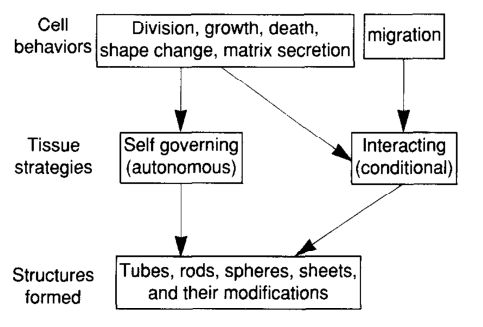
\includegraphics[scale=.38]{larsen}
\caption{Relationship between processes and biological
structures, excerpted from \cite{Larsen1992}. The six cell behaviors and two tissue strategies from which all morphology results.}
\label{fig:Larsen}
\end{wrapfigure}

\begin{longquote}
All morphology results from only
six cell behaviors and two tissue
strategies [Fig. 1]. Morphological
evolution occurs as a result of heritable modification of where and
when the six cell behaviors are
expressed. The six cell behaviors
contribute to many different tissue
structures; for example, cell death
is important in embryonic processes, such as the removal of cells
between human fingers to allow
their separation. Matrix secretion
is important in forming structures
like bone, but is also important in
more subtle aspects of development such as providing chemical
signs which guide migrating cells.
Migrating cells themselves can
help form an astonishing array of
structures including skeletal elements and muscles. However,
the cell behaviors perform their
roles according to one of two tissue
strategies.

In the self-governing (autonomous) strategy, sheets of cells,
known as epithelia, produce a variety of morphological structures,
including the four general types:
tubes, rods, spheres and sheets.
The power of self-governing
epithelial sheets to generate structures is well illustrated by imaginal
discs in \textit{D. melanogaster}. These are
sacs of cells, which originate as out-pockets from embryonic and early
larval epithelial sheets. During
larval life, localized cell divisions
produce disc-specific folds. At
metamorphosis, each disc turns
into a specific appendage, such as
a leg or antenna, chiefly through
changes in cell shape.

Unlike the self-governing strategy, a common tissue interaction or
conditional strategy employs mesenchyme cell migration and utilizes
interactions between mesenchyme
and epithelia. Mesenchyme cells
originate from epithelia through
cell detachment and migrate
through the epithelial basement
membrane. Their migratory path
and cell differentiation is directed
by interaction with overlying
epithelial cells. In vertebrate limb
development, signals from the
epithelium influence cell division
and differentiation in mesenchyme, while the mesenchyme
modulates cell division in the
epithelium. Thus, the tissue interaction strategy adds tissue level
controls to the development of the
four morphological structures from
which organisms are created. It is
important to realize that the tissue-
level controls produced by the
tissue interaction strategy may act
as developmental constraints to
evolution.
\cite{Larsen1992}
\end{longquote}

Dr. Larsen's view is summarised in her useful figure, adapted here as Fig. \ref{fig:Larsen}. Larsen is here concerned mainly with explaining the evolution of \textit{morphogenesis}, which is to say, the specialised functional roles that appear in the generated morphology are of less concern than the form-producing, spatial behaviours of the cells that produce them. While the SCBT is, of course, in conversation with the younger evolutionary developmental tradition (EDT), Larsen's perspective on tissue-level interactions is salutory. Harris' HJMEx are mainly about the dynamics of conceptually isolated cells, but what if he is wrong? In order to establish that, say, the inclusion of tissue-level effects improves the explanatory power of one of Harris' models, we have to be able to account for these effects in the first place. Moreover, Larsen has a clear perspective on tissue-level ``intermeshing properties": sometimes these are involved in tissue formation (autonomous), sometimes they aren't (interacting). At this point we should scrutinise these ``intermeshing properties" more carefully.

Since we know already that a tissue-level interactions are constituted by cellular interactions (which are in turn constituted by macromolecular zs $\mu$ing together in various ways). Let us first deal with the issue of the appropriate level of organisation for intermeshing properties specified by tissue-level HJMEx. We can imagine specifying all of these properties at the ``basement" level of macromolecular organisation in physico-chemical terms, and in so doing, specifying the tissue-level system that this web of macromolecular zs $\mu$ing would constitute. This would be a sort of macromolecular reduction, where we would try to explain Larsen's ``morphogenetic alphabet" \cite{Larsen1987} from the ground up. From the discussion above, and the polysemy we expect to encounter in our HJMEx, we can infer that in general, this would be futile. Moreover, ``Systems" approaches since Waddington have emphasized the organisation of the cell as a type of cybernetic bioreactor or factory. In Monod's memorable phrase, ``You have an exact logical equivalence between these two-the factory and the cell." The various feedback loops at this level are taken to constitute the general entity which is said to ``regulate" some cytoplasmic process. Although I think the cybernetic view is mistaken in significant ways, Waddington and Monod obviously understood perfectly well that molecular MEx would not make much sense as descriptions of isolated enzymes or chunks of signalling pathways-\textit{cum}-transcription networks. It may be possible to conceptually, if not experimentally\footnote{Obviously, enzyme biochemistry permits partial isolation of some kinds of macromolecular components \textit{in vitro}. The basic idea of synthetic chemistry was that biochemistry would allow the assembly of ``biological lego" in this biochemically reductionist sense. The fact that industrial bioprocess research has largely moved on from the idea of synthetic cells and is now focusing on ``\textit{in vitro} synthetic biology" is telling, given that this is nothing other than a description of the biochemical roots of the ``synthetic biology tradition".}, isolate these components and describe them in terms of their feedbacks on one another (as in the \textit{lac} operon), but these components only \textit{do} anything when installed in an appropriately regulated cybernetic cellular factory. Therefore, I take it that there is general agreement that a tissue-level HJMEx will focus on macromolecular phenomena at the level of the cell- where we cannot specify the macromolecular composition of some relevant system, we expect to encounter a statistical generalisation about what we take to be the activity of that macromolecular system operating \textit{at the level of whole cells}. 
 
 Let us briefly consider an example: we might postulate that in differentiating, a cell may change its transmembrane protein distribution over time, such that nearby cells are given a differentiation-promoting signal. If we want to represent this in our agent model, will we be looking for a description of the conformational states of transmembrane proteins, and the various models describing their interactions with neighbouring extracellular transmembrane domains? Only to the extent that such a description can inform us of what is happening at the \textit{overall} level of the cell, since we need to minimally hypothesize that such a protein is present in sufficient median concentration across the interacting membrane surface to have the pro-differentiation effect. As we may want to refer to a potentially polysemous macromolecular system (say, several separate pro-differentiation signalling pathways that separately contribute to this effect), the cell forms the ``ground floor" above the ``macromolecular basement". The fact that SCBT traditional explanations (and Harris' EHJMEx) are organised around the cellular ``ground floor" is thus unsurprising- being HJMEx, parts of the ``macromolecular basement" are not excavated, and other parts contain potentially chaotic polysemic macromolecular MEx. 
 
 We should further consider what this overall picture implies about higher levels of organisation before we move on. There are a few possible conceptual levels that are of less immediate interest: the lineage clearly matters, but in a retrospective, analytical sense, for instance. Tissue-level phenomena may meaningfully ``feed back" on the behaving cells which constitute those phenomena. Tissue-level phenomena will generally arise from composite action of cells, such that we expect to see population-level characteristics established at the level of the tissue, constituted by and feeding back upon the behaviour of the cells constituting those populations. If we bring in abstract ``tissue-level" effects, like a morphogen gradient, we understand this as a description of a population of cells, either locally or, in the case of tissue-interaction strategies, a second tissue-level mechanism meshing with the first. In the case of two tissue-level HJMEx interacting, we may expect one of these to be a highly abstract generalisation of a paired tissue, like a generalisation of the morphogen gradient, for instance. In this case the intermeshing property may be located in the cells of a local tissue responding to distant production of a signal. We understand that all of these generalisations are ``constituted" of cellular xs $\phi$-ing, which are in turn made of of macromolecular zs $\mu$-ing. It therefore seems that there is nothing in our selected modelling approach that would contradict the foregoing discussion of what we understand by HJMEx in the MBT.
 
 Having identified in my discussion of the \hyperref[SBE]{SBE} the agency or end-directedness of life as a good candidate for a counterinductive advance, and given my discussion of \hyperref[semiosis]{biosemiotics}, I repeat the suggestion here that semiotic phenomena must be accounted for in a more sophisticated manner than allowed for by the cybernetic approach. In particular, it should allow for phenomena to be divided between what the eminent philosopher of science Charles Sanders Peirce identified as ``dyadic", or asemiotic, brute facts, and those identified as ``triadic", or legitimately semiotic, habitual phenomena. Although considerations of space prevent a recapitulation of this argument here, we may simply note that the NetLogo agent modelling approach does not restrict us from making this kind of representation. This implies that we should be able to compare relatively asemiotic logics like those of Harris' EHJMex to those that include explicit representation of semiotic phenomena, given a global model that includes semiosis, since semiotic phenomena can simply be removed to express Harris' HJMEx as individual submodels within the global one. We therefore move to discuss the specifics of the statistical method involved in doing so.
 








\section{The Systems Biology Encounter - The Molecular Biological Tradition Under Impact}
\label{SBE}


\subsection{Historical sketch of the biological encounter with complexity}
\subsection{Explanatory Models in the Stem Cell Biology Tradition}




\section{"Metaphysical ingredients" encountered in MEx}
\subsection{Information theory}
\label{ITT}
The modern field of information theory (Information Theoretical Tradition, ITT) was essentially founded by the American polymath Claude Shannon during his work at Bell labs in the 1940s, building on cryptographic research, but elaborating a novel  fundamental theory of communication. Shannon used the thermodynamic concept of entropy to characterise the properties of entities involved in communication (sources, encoders, channels, etc).

It is important to immediately disabuse the reader of any notion that Shannon was at all concerned with meaning, or with the \textit{contents} of communication\footnote{Bioinformatically literate biologists are aware of this, but most of us do not routinely deal with formal definitions from information theory.}. Nowhere do the specific identities and contents of messages that habitually enter our minds when we think of biological communication enter Shannon's theory. Communication, for Shannon and for the electrical engineers for whom he was providing his theory, is an extremely broad concept. As Shannon's exegete Warren Weaver indicated in his classic introduction to Shannon's work, ``it may be desireable to use a [broad] definition of communication, namely, one which would include the procedures by means of which one mechanism (say automatic equipment to track an airplane and to computer its probably future positions) affects another mechanism (say a guided missile chasing this airplane)" \cite[p.10]{Shannon1963}. Therefore, Shannon's theory can be used to characterise some aspects of biological systems, but it must be clearly understood that ``information" refers to an abstract physical quantity and not to the lay definition concerning the specific contents of some communication.

Broadly speaking, the ITT has been applied to biological systems in two ways: analysis of biological communication and statistical measures of biological order.

\begin{enumerate}
\item{ITT analyses of biological communication} Shannon's 
\end{enumerate}

\subsection{RPC Fate Specification as a ``Stochastic" Process}
\label{stochastic}

Much of the complexity of this document is attributable to Harris' regular invocation of ``stochastic" and related adjectives to describe the behaviour of RPCs. This is what lead me to characterise the theory primarily in those terms- the Intrinsic Stochastic Effects (ISE) EHJMEx. It may not be immediately obvious why this should be the case; most scientists assume that they know what words like ``stochastic" and ``random" mean well enough to use them in rigorous technical publications. We may not be aware that there has been a sprawling debate on the meaning of these terms since the earliest statistical formulations begain to appear in the 19th century. However, even the simplest examples (as current today as they were in Laplace's time) reveal how difficult this topic can be.

If we consider the classic example of the coin flip, a process whose outcome we generally regard as being in some way ``stochastic" or due to ``chance", we immediately face the question of whether these descriptions refer to our inability to know the outcome of the process, or whether they refer to properties of the process itself. In other words, if we could specify the mechanics of the coin toss with sufficient precision, could we predict the outcome? This reflects two possible senses in which we may legitimately describe a process as ``stochastic": referring to an epistemic dimension (we may describe some process as stochastic because we are unable to predict its outcome \textit{a priori}), or referring to an ontological dimension (we describe the process as stochastic because this, in some way, describes how it \textit{really is} independent of our knowledge of it).

Complicating matters is the sheer number of implications that we tend to associate with ``stochasticity" and ``randomness". We may be saying something about the causal structure of an event with deep metaphysical implications. It is common to distinguish between ``deterministic" and ``stochastic" processes, as though ``stochastic" literally meant ``indeterministic"- something like the Copenhagen interpretation of quantum physics. We may mean something about the apparent disorderliness of a series of outcomes of some process, with mathematical and information theoretical implications. What is an apparently simple observation- cellular fate distribution in RPC lineages is ``stochastic", now seems to require at least a little clarification or interpretation.

Unfortunately, in Harris' case, a fulsome philosophically-inclined review of the ISE EHJMEx is yet to appear. We may attribute some of the difficulty encountered in interpreting the meaning of ``stochasticity" to the cramped style necessary in scientific reports. In general, we may say that stochasticity, for Harris, applies to at least the following entities:

\begin{enumerate}
\item The population-level phenomenal outcome of the RPC fate specification process (phenomenon P)
\item The overall behaviour of the macromolecular system whose operations produces these outcomes (mechanism S $\Phi$-ing)
\item The particular behaviour of some component of the macromolecular system, eg. stochastic expression of transcription factors (component x $\phi$-ing)
\item The statistical generalisations used to characterise relevant aspects of S $\Phi$-ing and x $\phi$-ing
\end{enumerate}

It is, moreover, hardly fair to expect Harris to be advancing a coherent theory about the ontological, objective basis of randomness or probability. Indeed, there is no real agreement on these concepts in probability theory or amongst the philosophers. Still, this leaves us in the awkward position of not knowing quite what the leading EHJMEx for retinal formation is actually saying about its explanandum. The EHJMEx is thus at risk of circularity- the explanandum (unpredictable variability in clonal outcomes, P) has as explanans a MEx containing an abstract mathematical model tuned to produce this unpredictable variability. This may, in other words, turn out to be a convoluted case of \hyperref[fitting]{model overfitting}, if the ``stochasticity" in question does not have a material biological referent. Before considering this, we need to define our terms more carefully to avoid the pervasive confusion mentioned above.

\subsubsection{Chance versus Randomness}
A commonplace belief is that randomness refers to outcomes produced by chance events. In an extensive and useful discussion, Antony Eagle reviews the evidence for this Commonplace Thesis, or \textbf{(CT)}\cite{Eagle2018}, drawing on discussions in the PTT. Importantly, he notes that chance and randomness are not identical, and that one can conceivably exist without the other. This, in effect, disproves the (CT)- it is very difficult to imagine how the two concepts can be directly related in this productive fashion. I will attempt a brief summary of Eagle's argument:

Chance is mainly used to refer to processes. Exemplars are coin flips and die rolls. We can think of these as ``single-case" probabilities that we take to inhere in the process. For instance, we may say that an evenly weighted coin has a .5 probability of returning a value of heads on a flip, even if it is only flipped once. That is, probabilities can be taken to be objective properties of individual instances of processes, and not only descriptions of the frequencies of the process' outcomes over many repetitions. This is closely related to the logical concept of ``possibility". If something is possible, it has a chance of occurring. However, possibility is a logical binary; something is either possible or impossible. A ``single-case" probability is understood as something like an objective feature of a system as a whole given its actual configuration and the relevant natural laws.  

Randomness, by contrast, mainly refers to process \textit{outcomes}. That is, randomness is a property of a series of outcomes of multiple instances of some process. It turns out to be challenging merely to define what a ``random" binary sequence might be (perhaps generated by a series of coin flips). However, in general, we may say that a random sequence of outcomes is one that cannot be generated by an description shorter than the sequence itself. That is, there is no set of rules that can generate a genuinely random sequence from a shorter sequence. In algorithmic information theory, the length of the ruleset required to produce some piece of information (like a sequence of measured outcomes) is called the Kolmogorov complexity of that object; if the Kolmogorov complexity of the object is equal to the object's length, the object definitionally has the property of algorithmic or Kolmogorov randomness.

Eagle produces numerous examples of the dissociability of these concepts, from which I have selected two concise illustrations:

\begin{longquote}
Chance Without Randomness

...

A fair coin, tossed 1000 times, has a positive chance of landing heads more than 700 times. But any outcome sequence of 1000 tosses which contains more than 700 heads will be compressible (long runs of heads are common enough to be exploited by an efficient coding algorithm, and 1000 outcomes is long enough to swamp the constants involved in defining the universal prefix-free Kolmogorov complexity). So any such outcome sequence will not be random, even though it quite easily could come about by chance. 

...

Randomness Without Chance

...

Open or dissipative systems, those which are not confined to a state space region of constant energy, are one much studied class [of the objects of deterministic classical physics- notably, biological systems are dissipative], because such systems are paradigms of chaotic systems ... the behaviour of a chaotic system will be intuitively random ... [t]he sensitive dependence on initial conditions means that, no matter how accurate our finite discrimination of the initial state of a given chaotic system is, there will exist states indiscriminable from the initial state (and so consistent with our knowledge of the initial state), but which would diverge arbitrarily far from the actual evolution of the system. No matter, then, how well we know the initial condition (as long as we do not have infinite powers of discrimination)\footnote{Note that this condition defines chaotic randomness as an epistemic, rather than ontological, feature of complex systems- a being with infinite powers of discrimination could predict the evolution of a complex classical system with perfect accuracy.}., there is another state the system could be in for all we know that will evolve to a discriminably different future condition. Since this divergence happens relatively quickly, the system is unable to be predicted ... Just as before, the classical physical theory underlying the dynamics of these chaotic systems is one in which probability does not feature. 
\cite{Eagle2018}
\end{longquote}

Therefore, the (CT) is untenable. Processes are ``chancy"; collections of process outcomes, ``trials", or instantiations are ``random". It is tempting to say that Harris is explaining random fate outcomes with descriptions of chancy processes occuring internally to RPCs. Let us examine whether this is plausible. 

\subsubsection{Chance in molecular mechanisms}
I turn first to consider what it might mean to describe the behaviour of a biological macromolecular system as ``chancy". Let us again distinguish between the ontological and epistemic dimensions of this description. There is a sense in which mechanisms S $\Psi$-ing could be said to be objectively chancy, and one in which the ``chancy" outcome reflects our ignorance of some source of variability in the process.

Eagle proffers two common lines of argument in favour of chanciness as an objective property of processes. The first is the notion of the ``single-case" probability mentioned above. The examples given are single coin flips, and the decay of single radioactive atoms, which are commonly taken to have chancy outcomes irrespective of anyone's beliefs about them. As Eagle notes, this is closely related to statistician's ideas about stable processes, or trials:

\begin{longquote}
It is the stable trial principle that has the closest connection with single-case chance, however. For in requiring that duplicate trials should receive the same chances, it is natural to take the chance to be grounded in the properties of that trial, plus the laws of nature. It is quite conceivable that the same laws could obtain even if that kind of trial has only one instance, and the very same chances should be assigned in that situation. But then there are well-defined chances even though that type of event occurs only once.

...

The upshot of this discussion is that chance is a \textit{process} notion, rather than being entirely determined by features of the outcome to which the surface grammar of chance ascriptions assigns the chance. For if there can be a single-case chance of $\frac{1}{2}$
for a coin to land heads on a toss even if there is only one actual toss, and it lands tails, then surely the chance cannot be fixed by properties of the outcome ‘lands heads’, as that outcome does not exist. The chance must rather be grounded in features of the process that can produce the outcome: the coin-tossing trial, including the mass distribution of the coin and the details of how it is tossed, in this case, plus the background conditions and laws that govern the trial. Whether or not an event happens by chance is a feature of the process that produced it, not the event itself. The fact that a coin lands heads does not fix that the coin landed heads by chance, because if it was simply placed heads up, as opposed to tossed in a normal fashion, we have the same outcome not by chance. Sometimes features of the outcome event cannot be readily separated from the features of its causes that characterise the process by means of which it was produced. 

\cite{Eagle2018}
\end{longquote}

Examining the example of the coin toss, we find a fairly simple answer to the question posed earlier: if we knew enough about the mechanics of the toss, could we predict its outcome? The answer is yes, we can- the statistician Persi Diaconis has built a coin tossing machine that reliably produces heads or tails \cite{Kestenbaum2004}. We therefore know that tightly controlling the mechanics of a coin toss allows us to treat this system as entirely deterministic, without any significant element of chance in the outcome. A coin toss is only chancy when the human doing it does not have full control over the mechanical parameters of the process. Conceptually, there is no \textit{a priori} reason why a coin-tosser should not be able to regularise the angular momentum of their thumb-flick by training with a strain gauge, place the coin on a stable surface allowing flicking, and achieve the same effect as the coin-tossing machine. In this case, Eagle's suggestion that ``[s]ometimes features of the outcome event cannot be readily separated from the features of its causes that characterise the process" seems obviously wrong- the ``chancy" element of coin tossing is fully separable from the rest of the coin tossing process, and replaceable with a non-chancy component.

If the foregoing argument is correct, it seems that the coin toss is an example of the epistemic, rather than ontological, dimension of chance. The process appears to be chancy, or random, because the human tossing the coin is not able to precisely control the mechanical parameters of the process. Indeed, as Diaconis notes, these epistemically-limited tossers do not actually produce unbiased random outcomes- human coin tosses come up as they were started slightly more often than with the obverse face \cite{Diaconis2007}.

Eagle's second example of an ``objective single-case chance", is the decay of a radioactive atom. This is a common method of making covert appeals to the second line of argument for objective chance, which is the existence of orthodox quantum theory. There is no known physical process whose parameters are thought to define the lifetime of individual radioactive atoms, in the way that there is a well-specified physical process that produces a particular coin toss outcome. Rather, this is an appeal to the Copenhagen theoretical principle that it is \textit{a priori} impossible to predict the lifetimes of individual atoms. As appeals to quantum theory to ground ``objective chance" in biological processes are becoming more common, let us consider whether a quantum theoretical explanation might plausibly underpin the ``stochasticity" of RPC fate specification.

\subsubsection{Quantum indeterminacy - Is relevant to the ISE?}
Eagle suggests that, because the Copenhagen interpretation of quantum physics has wide currency among physicists, the theory's implied indeterminacy of physical phenomena at the quantum level could ground ``objective chance". While common, this argument downplays the fact that quantum theory is not a homogenous scientific tradition. Unfortunately, a significant misrepresentation of the QTT's internal history has given rise to the impression that the Copenhagen theory is the unanimous or best articulation of quantum theory. We must briefly examine this misrepresentation before we can understand whether Eagle's argument makes sense.

The conventional history of the mid 20th-century QTT holds that John Stewart Bell, in the demonstration of his famous inequality, conclusively proved that deterministic (so-called ``hidden variable") theories of quantum mechanics were incorrect. As demonstrated (strangely, without any acknowledgement) in the very pages Eagle's argument appears in, this is a highly partisan and misleading view. Eminent Bohmian theorist Sheldon Goldstein conclusively demonstrates that Bell was an advocate of the deterministic Bohmian mechanical theory, and thought his famous inequality demonstrated that quantum phenomena could not be \textit{local}, not that they could not be \textit{deterministic}\cite{Goldstein2017}.

Indeed, Bohmian quantum mechanics are fully deterministic, describe all of the same phenomena as Copenhagen, and in several cases resolve problems that orthodox quantum theory cannot \cite{Goldstein2017}. We are not, therefore, facing unanimous expert consensus that there is objective chance at the quantum level. We rather have a situation where physical phenomena are adequately described by two different traditional theories, one of which takes its statistical generalisations to be descriptions of ontological indeterminacy (Copenhagen), and the other to reflect epistemic uncertainty about a determinate universe (Bohm). Moreover, there is no reason to prefer the Copenhagen approach, given that the Bohmian theory explains Copenhagen's paradoxical results ``without further ado"\cite{Goldstein2017}\footnote{Bizarrely, Copenhagen partisans claim that Bohmian mechanics is formally equivalent to the Copenhagen approach. If this is the case, chance is \textit{clearly} a function of model choices and not of any underlying ontological reality. However, Bohmian mechanics is, in fact, substantially more complete than its Copenhagen equivalent, which, by Eagle's (defective) logic, suggests reality is more likely to reflect the deterministic rather than the chancy approach.}, deals with empirically verified phenomena of physical and biological interest that Copenhagen does not (eg. electron tunneling), and was the preferred approach of the man who understood better than anyone his own results, JS Bell.

Therefore, Eagle's argument is incorrect. There is no reason to suppose that the existence of quantum theoretical models that posit objective chance is good evidence for the reality of objective chance. Moreover, there are good reasons to suppose that the converse is true. In sum, then, we may say that there is no reason to consider Harris' argument to refer to \textit{objective, ontological} chance, since the arguments for the existence of both single-case objective chance or quantum chance are weak and biologically irrelevant. Clearly, however, the \textit{epistemological} dimension of chance is in play here.

\subsubsection{Randomness in RPC fate specification}

Having dealt with how the concept of chance might apply to Harris' ISE EHJMEx above, let us consider how the term ``random" might relate to the process of RPC fate specification and differentiation. As introduced earlier, the technical meaning of ``randomness" pertains to sequences of process outcomes. The process outcomes Harris is concerned with are the temporally-arranged fate outcomes of some particular RPC lineage. Therefore, we must ask whether these sequences meet any reasonable technical definition of ``random".

Harris' own model proves that RPC fate outcomes are not algorithmically random. That is, the sequence of outcomes has a structure that can be meaningfully compressed by rules which produce typical RPC fate outcomes (Harris' mathematical models are such rule sets). One might object that Harris' meaning is that the particular rules which give rise to cellular fate ``choice" in his models involve random number generation. In this case, the claim is trivially about the model and not about the sequence of outcomes that is actually observed in zebrafish eyes. Indeed, all of Harris' later models \textit{axiomatically assume} a tripartite temporal structure to the differentiation process\footnote{That is, an early bias in RPC production is produced in these models by the a priori commitment to a ``rule" which results in early RPC production.}. This is precisely the type of sequential bias which allows efficient compression of a non-random sequence of outcomes by an algorithm. Therefore, Harris himself concedes that RPC fate specification is not an algorithmically random process\footnote{Having debunked the lay sense of ``random" being equivalent to ``chancy" above, there is no reason to consider these other, confused, non-technical definitions of randomness.}.

We should further note that the question of how ordered, which is to say, non-random processes like fate specification arise in biological systems is a fundamental question of the biological sciences. It has long been recognised that classical and quantum physical systems which have algorithmically random initial conditions do not spontaneously evolve to a state of order. In many ways, then, it is the extent to which variable sequences of outcomes like RPC fate specification \textit{depart} from algorithmic randomness which of interest when we are asking questions like ``how does the ordered structure of a retina arise from RPC activity?"

\subsubsection{Summary: ``Stochastic" or ``variable"?}

Above, I argue that the RPC fate specification process is not objectively chancy (since objective chance is an empirically unsupported concept), nor random (since the sequence of RPC lineage outcomes is structured and therefore non-random). What, then, should we make of the argument that this process is ``stochastic"? Let us consider the forceful argument of the great Bayesian statistician Edwin Thompson Jaynes:

\begin{longquote}
 ``Belief in the existence of ‘stochastic processes’ in the real world; i.e. that the property of being ‘stochastic’ rather than ‘deterministic’ is a real physical property of a process, that exists independently of human information, is [an] example of the mind projection fallacy: attributing one’s own ignorance to Nature instead. The current literature of probability theory is full of claims to the effect that a ‘Gaussian random process’ is fully determined by its first and second moments. If it were made clear that this is only the defining property for an abstract mathematical model, there could be no objection to this; but it is always presented in verbiage that implies that one is describing an objectively true property of a real physical process. To one who believes such a thing literally, there could be no motivation to investigate the causes more deeply than noting the first and second moments, and so the real processes at work might never be discovered. This is not only irrational because one is throwing away the very information that is essential to understand the physical process; if carried into practice it can have disastrous consequences. Indeed, there is no such thing as a ‘stochastic process’ in the sense that the individual events have no specific causes." \cite{Jaynes2003}
 \end{longquote}
 
It is important to emphasize that the utility of stochastic modelling techniques should not be taken to suggest that on some level the modelled phenomenon is actually, i.e. irreducibly, random and without causal structure. When speaking of biological ``randomness" or ``stochasticity", biologists rarely precisely define what is meant by these terms. This vagueness sometimes arises from or results in a theoretical deficit where properties of statistical models are understood to directly reflect the system being modelled; the scientist has failed to heed Korbzysky's dictum insisting that ``a map \textit{is not} the territory it represents, but, if correct, it has a \textit{similar structure} to the territory, which accounts for its usefulness" \cite{Korzybski2005} (italics in original). The ``structural similarity" here is between the model's outcomes and the collection of actually-observed population outcomes, \textit{not} the underlying biological process giving rise to measured outcomes.

However, it would be trivial and a violation of my commitment to the principle of charity to dismiss Harris' argument on this basis. While I do believe that Harris has fallen into the ``mind-projection fallacy" James excoriates above, we must ask how this occurred. What was the attraction of this fallacious explanation in the first place? I suggest that Harris appeals to stochasticity as an explanation for \textit{variability} in fate outcomes. Harris describes his work as an attempt to explain how variable clonal outcomes could give rise to an ``invariant" retina. We want to know how it is that variable clonal outcomes are produced and what this phenomenon's significance is to overall retinal formation. The value of Harris' ISE EHJMEx, I suggest, lies in its emphasis on the unpredictable variability of RPC lineage outcomes. I have suggested a scheme for identifying possible sources of biological variability in a \hyperref[variability]{separate section} of this chapter.

\subsection{Biological Variability}
\label{variability}
As I have argued in section \ref{stochastic}, there are no good reasons to think that differential outcomes in biological systems are a result of some fundamental, ontological randomness. I share Jaynes' objection to this argument- the result is that the so-described phenomenon is understood to be, on some level, causeless. We are nevertheless left with the fact of unpredictable biological variability. Of course, observations documenting these variable phenomena are perplexing in the context of the pervasive Monodian conventional view, to wit, that cells are logically equivalent to \hyperref[cybernetics]{cybernetic chemical factories}. In a factory, process control is fundamentally about managing variability. Normally, we want to produce some regular sequence of outcomes for a production line with minimal variability. The chemical factory metaphor requires modification when applied to the context of Harris' work, however\footnote{This modification is a logical consequence of the transposition of Monod's cybernetic metaphor for bacterial operons to a multicellular system.}. The products we are interested in are cellular fate outcomes themselves. Starting with an aggregate of similar (genetically, if not epigenetically, identical) RPCs, a \hyperref[hierarchy]{specification hierarchy} emerges. To re-fit the industrial metaphor to the context, the chemical-factory equivalent would be to explain how one can start with a factory that makes machine tools and end with a group of factories that make the diverse chemical products of a highly networked modern chemical industrial sector. In the absence of any central planner, how might the ontogenesis of such an industry take place? What are the factors that give rise to the ``decision" to build one type of factory or another, and how do we explain the apparent increase in networked complexity and functional specialisation? What is the source of this apparent scaffolding novelty, and how can we explain the specific outcomes that we observe?\footnote{The factory metaphor makes it obvious that this type of question has far more to do with developmental or historical economics than it does with cybernetic process control of petrochemical cracking vessels or fermenters. Aside from Markoff chain theory, biologists have generally avoided methods used to study systems where outcomes heavily depend on the history of the system and related contingencies, probably because of the lack of scientific prestige associated with many of these formalisms ("soft science"). Nonetheless, it is hard to see how one can explain tissue development exclusively in terms of control of cell-internal processes- to attempt this is like trying to explain the historical evolution of the biotechnological industry in terms of the PID controllers it uses to run its fermenters. This will be, at best, a partial and highly misleading account.}

Indeed, an explanation of biological variability is, alongside explaining the emergence of biological order, the fundamental task of the biological sciences. Harris has bravely advanced a theory that has, at times, referenced different possible sources for the variability observed in 

\subsubsection{Noise}

\subsection{Time}
\label{time}
\subsection{Semiosis, Meaning}
\label{semiosis}
\subsection{Emergence, self-organisation}
\label{emergence}
\subsection{Scale Hierarchies, Specification Hierarchies}
\label{hierarchy}
\subsection{Waddington's topological model of development}
\label{Waddington}
\begin{longquote}
C. H. Waddington was one (and almost certainly the
best remembered) of the embryologists who so profited. He
wrote: “During the recent war, engineers attained some fa-
cility in designing machines to carry out tasks which earlier
generations would have considered beyond the capacities of
anything but an intelligent being . . . The ideas suggested
by these self-regulating mechanisms are both very relevant
to biology and rather novel.” 28 Waddington himself worked
in the Operation Research Section of the Royal Air Force
Coastal Command, and it was from his own experience and
from that of his friends in self-steering gunnery that he
learned to draw the analogy which was to become increas-
ingly familiar in the cybernetics of the 1950s and 1960s: “The
behaviours of an automatic pilot, of a target-tracking gun-
sight, or of an embryo, all exhibit the characteristics of an
activity guided by a purpose.” 29 Indeed, it was at this time,
and in this context, that his work on canalization began. 30
In Waddington’s first introduction of the term, he
wrote, “The main thesis is that developmental reactions as
they occur in organization submitted to natural selection,
are, in general, canalized. That is to say, they are adjusted so
as to bring about one definite end result regardless of mi-
nor variations in conditions during the course of the reac-
tion.” In his view, canalization is built into the organism by
natural selection as a consequence of its obvious advan-
tages: “It ensures the production of the normal, that is, op-
timal type in the face of the unavoidable hazards of exis-
tence.” 31 Canalization was a term Waddington had borrowed
from his reading of Alfred North Whitehead, and the con-
cept clearly accorded with much of his own prewar thinking
about “epigenetic landscapes.” 32 But it was only after the
war that he began to envision the possibility of a theoretical
account of such characteristic features of biological organi-
zation. An explanation of “developmental canalization,” he
wrote, requires supplementing conventional gene theory
with an “epigenetic theory”—one in which discrete and sepa-
rate entities of classical genetics would be displaced by col-
lections of genes which could ‘lock in’ development through
their interactions.” 33 In other words, an account of develop-
mental stability needs to be sought in the complex system
of reactions that make up the developmental process.
The search for quantitative models displaying such be-
havior underlay much of Waddington’s theoretical efforts
well into the 1970s. However, he soon concluded that the
particular models developed by Ross Ashby and other cyber-
neticians on self-organizing systems were not really appro-
priate to biological development. Instead, he concentrated
on feedback models of cross-reacting systems of metabolic
reactions. Yet he did not have a great deal of success with
these models. Indeed, it is not his theoretical work but the
experimental work from his laboratory in the 1940s and ’50s
that now, with the benefit of hindsight, attracts the most in-
terest.
\cite[p.117-119]{Keller2000}
\end{longquote}

\begin{figure}
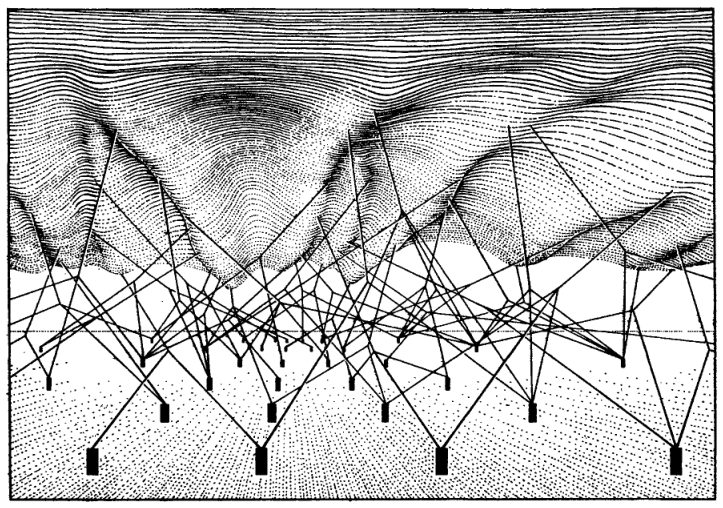
\includegraphics[scale=.5]{Waddington}
\centering
\caption{The complex system of interactions underlying the epigenetic landscape, excerpted from \cite{Waddington1957}.
The pegs in the ground represent genes; the strings leading from
them the chemical tendencies which the genes produce. The
modelling of the epigenetic landscape, which slopes down from
above one's head towards the distance, is controlled by the pull
of these numerous guy-ropes which are ultimately anchored to
the genes.}
\label{fig:Waddington}
\end{figure}


\subsection{Morphogenetic fields}
\subsection{Physical explanations}
\label{physex}



\section{Implications of Limits in Theory and Practice For Model Selection}
\label{limits}
\subsection{Nicholas Rescher's Account of Scientific Progress}

\subsection{Implications of Theoretical Limits of Science}
\label{theorylimits}
\subsection{Implications of Thermoeconomic Limits of Science}

\subsection{Practical computational limits}
\label{complimits}


